% =============================================================================
%  Dissertação de Mestrado — Instituto Superior Técnico
%  Compilar:  latexmk -xelatex main.tex
%  Limpar:    latexmk -c
% =============================================================================
\documentclass{istdissertacao}

\addbibresource{referencias.bib}
% =============================================================================
%  macros.tex — atalhos para símbolos usados repetidamente
%  Vantagem: se mudar a notação, muda-se aqui e propaga para toda a tese.
% =============================================================================

% --- cinemática ---------------------------------------------------------------
\newcommand{\pt}{p_{\mathrm{T}}}
\newcommand{\ptjet}{p_{\mathrm{T}}^{\mathrm{jet}}}
\newcommand{\pT}{p_{\mathrm{T}}}
\newcommand{\dR}{\Delta R}
\newcommand{\kt}{k_{\mathrm{T}}}
\newcommand{\antikt}{anti-$\kt$}
\newcommand{\CA}{Cambridge/Aachen}

% --- observáveis do plano de Lund --------------------------------------------
\newcommand{\lnkt}{\ln \kt}
\newcommand{\lninvdR}{\ln(1/\dR)}
\newcommand{\dpsi}{\Delta\psi_{12}}
\newcommand{\tauf}{\tau_{\mathrm{f}}}
\newcommand{\zcut}{z_{\mathrm{cut}}}

% --- energia do feixe: definir uma vez, usar em todo o lado -------------------
\newcommand{\SIvalue}{13}          % <<< ajustar ao dataset usado (7, 8 ou 13)
\newcommand{\roots}{\sqrt{s} = \SIvalue~\mathrm{TeV}}

% --- utilitários --------------------------------------------------------------
\newcommand{\GeV}{\,\mathrm{GeV}}
\newcommand{\TeV}{\,\mathrm{TeV}}



% ---------------------------------------
% IDIOMA DO CORPO DA TESE
% A classe fixa os nomes em português (Índice, Quadro, Figura, ...).
% Se escrever a tese em inglês, descomente o bloco abaixo.
% ---------------------------------------
% \renewcommand{\contentsname}{Contents}
% \renewcommand{\listfigurename}{List of Figures}
% \renewcommand{\listtablename}{List of Tables}
% \renewcommand{\bibname}{References}
% \renewcommand{\appendixname}{Appendix}
% \captionsetup[table]{name=Table}
% \captionsetup[figure]{name=Figure}
\newcommand{\ISTbodylang}{english}
% \newcommand{\ISTbodylang}{portuguese}   % <<< comentar se usar o bloco acima

% ---------------------------------------
% DADOS DA DISSERTAÇÃO  <<< PREENCHER >>>
% ---------------------------------------
\titulodissertação{Exploring Jet Substructure in Public LHC Data}
%\subtitulodissertação{Subtítulo}
\autordissertação{Alexandre Maria Neves de Barbosa Mendonça}
\graudissertação{Mestre}
\cursodissertação{Engenharia Física Tecnológica}
\orientadoresdissertação{Professor Doutor José Guilherme Teixeira de Almeida Milhano\\Professor Doutor Nuno Filipe da Silva Fernandes de Castro}
\presidentejuri{Professor Doutor Nome Completo}
\vogaisjuri{Professor Doutor Nome Completo\\Doutor Nome Completo}
\datadissertação{Outubro de 2026}
% \imagemcapa{figuras/imagem-capa.pdf}   % altura máxima: 5 cm
% \logoacademia{figuras/logo-academia.pdf}
% \versaodefinitiva                      % descomentar na entrega final

\usepackage{fancyhdr}
\fancypagestyle{plain}{%
  \fancyhf{}%                        % limpa tudo
  \fancyfoot[R]{\thepage}%           % número no rodapé, à direita
  \renewcommand{\headrulewidth}{0pt}%
  \renewcommand{\footrulewidth}{0pt}%
}
\usepackage{tikz}
\usetikzlibrary{positioning,fit,arrows.meta,backgrounds}
\usepackage{xltabular}

\pagestyle{plain}

\begin{document}
\selectlanguage{english}

\capadissertação
\declaracao

\frontmatterIST

% ---------------------------------------
% PÁGINAS PRELIMINARES
% Resumo (PT) e Abstract (EN) são ambos obrigatórios, seja qual for o idioma
% escolhido para o corpo da tese. Máximo 250 palavras cada, 4 a 6 palavras-chave.
% ---------------------------------------

\chapter*{Agradecimentos}
\addcontentsline{toc}{chapter}{Agradecimentos}

Ao Professor Guilherme Milhano e ao Professor Nuno Castro, meus orientadores,
agradeço a confiança e a oportunidade que me deram para explorar este tema e
a disponibilidade que demonstraram desde o início deste projeto. Muitas discussões
e sugestões foram feitas ao longo deste trabalho e, sem elas, este não seria nem de
perto o mesmo. Agradeço também as indicações sobre o meu percurso académico, que sem
dúvida mudaram e mudarão a minha pessoa, e com toda a certeza para algo melhor.

Ao LIP, e em particular ao LIP Minho e ao grupo de Fenomenologia, agradeço o
acolhimento e o ambiente de trabalho que ajudaram esta tese a tornar-se possível.
Agradeço também ao LIP e à INCD pela disponibilização de recursos computacionais,
sem os quais nada desta tese estaria feito, e à Colaboração CMS pela
publicação dos dados e das simulações em que todo este trabalho assenta.

À minha mãe, um especial agradecimento, pois é a ela que dou graças por estar aqui
neste momento, por me ter apoiado sempre nas minhas escolhas tanto académicas como
pessoais e por me ter tornado nesta pessoa que teve o prazer de ter feito esta tese e
que quer continuar a fazer mais. Esta tese é também tua.

\chapter*{Resumo}
\addcontentsline{toc}{chapter}{Resumo}

As correlações de spin colineares, induzidas pela polarização linear dos gluões
intermédios na cascata partónica, produzem uma modulação azimutal entre
ramificações sucessivas nos jatos. Este trabalho estuda-as com dados do CMS Open
Data, de colisões protão-protão a $\sqrt{s} = 13$~TeV registadas em 2016, e a
respetiva simulação \textsc{Pythia}~8. Construiu-se uma cadeia de análise
reprodutível para observar a modulação do ângulo $\dpsi$ entre os planos das duas
ramificações mais duras na desaglomeração de Lund de jatos com $\pt > 700$~GeV e a
modulação azimutal do correlador de energia de três pontos. Como os canais
$g \to q\bar{q}$ e $g \to gg$ contribuem com sinais opostos, desenvolveu-se uma
seleção em duas etapas com redes neuronais para enriquecer as amostras em
ramificações $g \to q\bar{q}$, identificadas na simulação com o algoritmo de
neutralização de sabor intercalada. Sem seleção, obteve-se
$\langle \cos 2\dpsi \rangle = -0.078 \pm 0.003$ nos dados, em acordo com a
simulação. Na simulação, a seleção intensifica a modulação de $-0.12$ para
$-0.27$ quando a pureza sobe de $0.18$ para cerca de metade, e os dados
acompanham-na dentro da sua precisão. A decomposição por canal mostra, contudo,
que todas as classes contêm uma componente importante sem origem no spin e que a
seleção desloca a modulação de cada classe, pelo que a modulação selecionada não
pode ser atribuída apenas ao canal $g \to q\bar{q}$. O correlador de energia
apresenta uma pequena modulação positiva, quase insensível ao canal. Estes
resultados são consistentes com a recente observação do CMS, mas estabelecer as
correlações de spin requer uma previsão sem elas, processada pela mesma seleção.

\vspace{1em}
\textbf{Palavras-chave:} Subestrutura de jatos, Correlações de spin
colineares, Polarização do gluão, Plano de Lund, CMS Open Data, Aprendizagem
automática

\cleardoublepage
\selectlanguage{english}
\chapter*{Abstract}
\addcontentsline{toc}{chapter}{Abstract}

Collinear spin correlations, induced by the linear polarisation of intermediate
gluons in the parton shower, produce an azimuthal modulation between successive
splittings inside jets. This work studies them using CMS Open Data datasets, created
from proton-proton collisions at $\sqrt{s} = 13$~TeV recorded in 2016 and the
corresponding \textsc{Pythia}~8 simulation. A reproducible pipeline was built 
in order to observe the modulation of the angle $\dpsi$ between the planes of the
two hardest splittings in the Lund declustering of jets with $\pt > 700$~GeV, and
the azimuthal modulation of the three-point energy correlator. Given that 
the $g \to q\bar{q}$ and $g \to gg$ channels contribute with opposite signs, a
two-stage neural-network selection was developed to enrich the samples in
$g \to q\bar{q}$ splittings, which were labelled in simulation using the
interleaved flavour neutralisation algorithm. Before any selection was done, the value
$\langle \cos 2\dpsi \rangle = -0.078 \pm 0.003$ was obtained in data, in agreement with the
simulation. The implemented selection strengthens the modulation from $-0.12$ to $-0.27$ in
simulation as the purity rises from $0.18$ to about one half, and the data follow
the simulation wherever their precision allows. The decomposition by channel
shows, however, that every class carries a large non-spin component and that the
selection shifts the modulation of each class, so the selected modulation cannot
be interpreted as that of the $g \to q\bar{q}$ channel alone. The energy
correlator shows a small positive modulation, nearly insensitive to the channel.
These results are consistent with the recent CMS observation, but establishing the
spin correlations requires a prediction without them, processed through the same
selection. 


\vspace{1em}
\textbf{Keywords:} Jet substructure, Collinear spin correlations, Gluon
polarisation, Lund jet plane, CMS Open Data, Machine learning

\cleardoublepage
\selectlanguage{\ISTbodylang}

\tableofcontents

\cleardoublepage
\phantomsection
\addcontentsline{toc}{chapter}{\listtablename}
\listoftables

\cleardoublepage
\phantomsection
\addcontentsline{toc}{chapter}{\listfigurename}
\listoffigures

\chapter*{List of abbreviations}
\addcontentsline{toc}{chapter}{List of abbreviations}

\begin{xltabular}{\textwidth}{@{}lX@{}}
\multicolumn{2}{@{}l}{} \\[4pt]
AK8     & Jets clustered with the anti-$\kt$ algorithm and $R = 0.8$ \\
ALICE   & A Large Ion Collider Experiment \\
AOD     & Analysis Object Data \\
ATLAS   & A Toroidal LHC ApparatuS \\
C/A     & Cambridge/Aachen algorithm \\
CERN    & European Organization for Nuclear Research \\
CMS     & Compact Muon Solenoid \\
CMSSW   & CMS Software \\
CP5     & \textsc{Pythia}~8 tune derived by CMS \\
DGLAP   & Dokshitzer-Gribov-Lipatov-Altarelli-Parisi \\
DNN     & Deep neural network \\
ECAL    & Electromagnetic calorimeter \\
EEEC    & Three-point energy correlator \\
FWLite  & CMS Framework Lite \\
HCAL    & Hadronic calorimeter \\
HLT     & High-Level Trigger \\
IFN     & Interleaved flavour neutralisation \\
IRC     & Infrared and collinear \\
LHC     & Large Hadron Collider \\
LHCb    & Large Hadron Collider beauty \\
LIP     & Laboratório de Instrumentação e Física Experimental de Partículas \\
MiniAOD & Reduced version of the AOD format, retaining the particle-flow candidates \\
NanoAOD & Further reduced version of the AOD format, without constituent information \\
PR      & Precision-recall \\
PUPPI   & Pileup per particle identification \\
QCD     & Quantum Chromodynamics \\
ReLU    & Rectified linear unit \\
ROC     & Receiver operating characteristic \\
\end{xltabular}


\mainmatterIST

\chapter{Introduction}
\label{cap:introducao}

\section{Context and motivation}
\label{sec:motivacao}

The Large Hadron Collider (LHC) at CERN produces the highest energy proton-proton
collisions ever achieved in a laboratory and, with them, an enormous sample of
strongly interacting final states. The majority of these collisions are governed
by Quantum Chromodynamics (QCD), the gauge theory of the strong interaction. The
comprehension and study of these collisions are not only a prerequisite for
suppressing backgrounds in searches for new phenomena, but also allow the
structure of the hadronic final state to be examined and compared to theory
directly, at scales where the coupling is weak enough for perturbation theory to
be applied and yet the dynamics still remain rich.

The most prominent objects in these final states are jets. Jets are collimated
sprays of hadrons that emerge from the fragmentation of high-energy quarks and
gluons. A jet is not a fundamental object but instead a definition. A clustering
algorithm specifies which detector inputs are grouped together, and a
recombination scheme specifies how momentum is assigned to the result. This
defines a jet, from which an interesting and important question then arises. What
does the radiation inside the jets look like? This domain is called jet
substructure, which over the past decade has grown from a collection of tagging
tools into a precision probe of QCD dynamics in its own right.

In order to organise and look at the internal structure of a jet, one can use the
Lund jet plane~\cite{Dreyer:2018nbf}. The Lund jet plane is a two-dimensional map of a
jet's branching history on which soft, collinear, and non-perturbative regions of
QCD radiation occupy distinct territories. This map records where the jet's
internal emissions occur, but it sets aside an intriguing piece of information,
the orientation of each splitting relative to the one before. This orientation is
not random. Through the linear polarisation of intermediate gluons, successive
splittings are correlated in their relative azimuthal angle, producing a
characteristic modulation in the distribution of that angle. This is a genuine
quantum interference effect which survives only because the intermediate gluon is
described by an amplitude rather than a probability, and it is absent from any
picture that treats successive emissions as independent classical branchings.

These collinear spin correlations are well understood theoretically and are
implemented in modern parton shower algorithms, yet establishing them in
collision data has proved difficult. They were observed only recently by the CMS
Collaboration, in jets enriched in $g \to q\bar{q}$ splittings~\cite{CMS:2026jnt}.
The main difficulty is that the effect carries opposite signs in different
splitting channels. The $g \to q\bar{q}$ and $g \to gg$ channels contribute with
opposite sign, so a measurement that sums all channels sees the two contributions
partially cancel. This interference is not absent from such an inclusive
measurement. It is diluted, and the apparent size reflects the accidental flavour
composition of the sample rather than the strength of the underlying physics. The
measured distributions also receive contributions unrelated to the spin, which a
measurement must be able to separate from the effect.

This is the obstacle the present work addresses. A meaningful measurement of the
effect requires knowing which splitting produced each emission. However, the
flavour of an individual splitting inside a jet is not directly observable and
must be inferred. Working entirely on public CERN Open Data~\cite{CERNOpenData}, more
precisely with CMS Open Data~\cite{CMSOpenDataGuide}, this dissertation builds a
reproducible pipeline from the released samples through Lund declustering to the
azimuthal spin observable, and introduces a flavour selection that enriches the
selected samples in the $g \to q\bar{q}$ channel. The resulting modulation is
reported as a function of the threshold of that selection, with the purity of
each selected sample determined in simulation. The behaviour of each channel under
the selection is also studied in simulation, which shows to what extent the
modulation of a selected sample reflects that of the $g \to q\bar{q}$ channel.

The Lund declustering angle $\dpsi$ is not the only way to reach this effect. The
same $\cos 2\psi$ modulation also imprints itself on the flow of energy within a
jet, and can be accessed through a three-point energy correlator, which probes the
relative azimuthal orientation of energy deposited by triplets of particles
without reference to any clustering history. The two observables are
complementary. One reads the effect from the reconstructed branching sequence, the
other from the energy flow directly, and each carries a different exposure to the
choices and imperfections of the measurement. This work develops both, treating
the Lund observable as the primary measurement and the energy correlator as a
complementary probe of the same underlying physics.

The fact that this analysis rests on public data is not incidental. The CERN Open
Data Portal has made it possible for work outside the experimental
collaborations to produce meaningful results and to carry out genuinely new
measurements. The present work is intended as a contribution in that spirit. It
builds an end-to-end pipeline from the CMS collision data and simulation to the
final measurements, establishing along the way a workflow for accessing, handling
and measuring with CMS Open Data, whose code is publicly
available~\cite{Mendonca:CMSJetSubstructure}.

\section{Objectives}
\label{sec:objetivos}

The main aim of this dissertation is to study collinear spin correlations in QCD
jets using public LHC data and to establish the flavour selection that such a
measurement requires in order to be meaningful. For the purpose of achieving that
goal, the work is organised around a sequence of objectives. The first is to build
a reproducible pipeline over CERN Open Data samples capable of extracting the
necessary variables to begin a jet substructure analysis. This means that the data
samples must contain jet constituent information, thus, the data format chosen must
retain that level of detail, ruling out the more compact samples in favour of one
that preserves per-constituent quantities.

With that pipeline in place, the second objective is to construct the primary and
secondary Lund jet planes and to verify that they reproduce the known features of
QCD radiation, since this agreement is what establishes that the declustering is
sound before any finer observable is built on top of it. Following that, the third
objective is to implement the azimuthal observable $\dpsi$ between the hardest
primary and secondary branchings, with the grooming condition $z > 0.1$, and to
study its inclusive distribution before attempting to sharpen it. The same
objective includes the azimuthal modulation of the three-point energy correlator,
implemented as a complementary probe that does not rely on the declustering.

The fourth objective is the central one, and the point at which this work departs
from a purely inclusive analysis. Because the spin-interference signal carries
opposite signs in the $g \to q\bar{q}$ and $g \to gg$ channels, an inclusive
measurement dilutes it. Enriching the sample in a single channel is therefore not
a refinement but a precondition for observing the effect of that channel. This
objective is thus to develop a flavour selection capable of enriching the
$g \to q\bar{q}$ channel, and to quantify both how well it performs and how pure a
sample it can reach in principle. The fifth objective builds directly on it. It is
to measure $\langle \cos 2\dpsi \rangle$ as a function of the flavour selection,
in data and in simulation, and to determine to what extent the modulation of the
selected samples reflects that of the $g \to q\bar{q}$ channel.

Finally, the work aims to identify the sources of systematic uncertainty affecting
this measurement and the dominant limitations of the approach, so that the
extensions it opens up can be set out on solid ground.

\section{Thesis outline}
\label{sec:estrutura}

Chapter~\ref{cap:estado-da-arte} develops the theoretical material on which the
measurement rests, such as the elements of QCD relevant to jet formation, the
definition and reconstruction of jets and the algorithms used to build and
decluster them, the Lund jet plane, and the origin of collinear spin correlations
together with the two observables through which this work accesses them.
Chapter~\ref{cap:metodos} turns to the data and the analysis, and covers the CERN
Open Data resources and the CMS detector, the data format and dataset used, and
the pipeline that runs from the released samples through Lund declustering to the
azimuthal observable, the flavour selection, and the treatment of systematic
uncertainties. Chapter~\ref{cap:resultados} presents the validation of the
pipeline and the measurements of both observables, and discusses the results in
the light of the expectations set out in Chapter~\ref{cap:estado-da-arte} and of
the CMS measurement. Finally, Chapter~\ref{cap:conclusoes} returns to the
objectives of Section~\ref{sec:objetivos}, states what has been established and
with what confidence, and outlines the extensions that the present framework makes
possible. Appendix~\ref{anexo:b} collects the numerical values behind the figures
of Chapter~\ref{cap:resultados}.
\chapter{Theoretical Background}
\label{cap:estado-da-arte}

\section{Quantum Chromodynamics}
\label{sec:qcd}

Quantim Chromodynamics (QCD) is the quantum field theory of the strong interaction,
a non-Abelian gauge theory built on the colour symmetry group $SU(3)$ \cite{Ellis:1996mzs}.
Its fundamental degrees of freedom are quarks, which carry colour charge, and gluons,
the gauge bosons that mediate the interaction. The non-Abelian character of the theory
has a decisive consequence absent from Quantum Electrodynamics. The gluons themselves
carry colour, and therefore couple directly to one another. To a large extent, the
dynamics of the strong interaction are the dynamics of this gluon self-coupling, and
the two properties of QCD that govern everything in this chapter both follow from it.

\subsection{Asymptotic freedom and confinement}

The first property is asymptotic freedom. The strong coupling $\alpha_s$ decreases
as the momentum transfer of an interaction increases, so that at the high scales 
probed in LHC collisions the quarks and gluons interact weakly and perturbation
theory applies \cite{Gross:1973id,Politzer:1973fx}. The running of the coupling
is captured at leading order by

\begin{equation}
    \alpha_s(Q^2) = \frac{\alpha_s(\mu^2)}
    {1 + \alpha_s(\mu^2)\,\dfrac{33 - 2 n_f}{12\pi}\,\ln\!\dfrac{Q^2}{\mu^2}},
    \label{eq:running}
\end{equation}

where $Q$ is the scale of the process, $\mu$ a reference scale, and $n_f$ the
number of active quark flavours. The positive sign of the coefficient
$33 - 2n_f$, which holds for any physical number of flavours, is what makes the
coupling fall at large $Q$.  It is a direct imprint of the gluon self-interaction,
and its discovery established that a peturbative treatment of hard processes is
justified. It is convenient to trade the reference scale for a single dimensionful
constant $\Lambda_{\mathrm{QCD}}$, the scale at which the peturbative coupling formally
diverges, of an order of a few hundered MeV. In terms of it the coupling is small for
$Q \gg \Lambda_{\mathrm{QCD}}$ and grows strong as $Q$ approaches it.

This growth is the second property called confinement. At low momentum transfer
$\alpha_s$ becomes large and colour-charged particles cannot be isolated. A
quark or gluon produced in a hard scattering does not propagate freely to a detector,
because as it separates from other colour charges, the energy stored in the colour field
between them grows with distance until it becomes energetically favourable to create
a new quark-antiquark pairs from the vacuum. The original parton is thereby
dressed into a spray of colour-neutral hadrons. This is why the strongly interacting
final state reaches the detector not as partons but as the collimated sprays introduced
in Chapter \ref{cap:introducao}, and why any comparison between a peturbative
calculation and a measurement must bridge the divide between the patronic and hadronic
descriptions.

\subsection{Soft and collinear radiation}

The bridge between the hard parton and the observed hadrons is built from
successive emissions, and the pattern of those emissions is far from uniform.
When a parton radiates a gluon, the emission probability at first order in the
coupling takes the schematic form

\begin{equation}
  d\mathcal{P} \;\propto\; \frac{2\alpha_s C}{\pi}\,
  \frac{d\theta}{\theta}\,\frac{dE}{E},
  \label{eq:soft-collinear}
\end{equation}

where $E$ and $\theta$ are the energy and emission angle of the radiated gluon
and $C$ is a colour factor. The two factors carry the characteristic structure of
QCD radiation. The factor $d\theta/\theta$ diverges as $\theta \to 0$ meaning that
emmissions are enhanced when the gluon is radiated close to the direction of its emmiter.
This is known as the collinear divergence. The factir $dE/E$ diverges as $E \to 0$
meaning that emissions are enchanced when the gluon is soft. This is known
as the soft divergence. Together they mean that a hard parton radiates predominantly
softly and at small angles, and that number of such emissions is,
in a precise logarithmic sense, large.

The collinear structure is described more completely by the 
Dokshitzer–Gribov–Lipatov–Altarelli–Parisi (DGLAP) splitting
functions \cite{Ellis:1996mzs}, which give the probability that a parton of one type splits into two,
as a function of the momentum fraction $z$ carried by one of the products. For
the three splittings relevant to this work they read, at leading order,

\begin{align}
  P_{q \to qg}(z) &= C_F\,\frac{1 + z^2}{1 - z}, \label{eq:Pqq}\\[4pt]
  P_{g \to gg}(z) &= C_A\,
    \left[ \frac{z}{1-z} + \frac{1-z}{z} + z(1-z) \right], \label{eq:Pgg}\\[4pt]
  P_{g \to q\bar{q}}(z) &= T_R\,\left[ z^2 + (1-z)^2 \right], \label{eq:Pgq}
\end{align}

with colour factors $C_F = 4/3$, $C_A = 3$ and $T_R = 1/2$. The distinction
between the gluon splitting channels of Eqs. \eqref{eq:Pgg} and \eqref{eq:Pgq},
one producing a pair of gluons and the other a quark-antiquark pair, will
prove central. The two channels differ not only in these rates but in the spin
structure of their emissions, and it is that difference which the spin
observables of Section \ref{sec:spin} are designed to probe.

These divergences are not a pathology. They are integrable, and in any physical,
infrared-safe observable the divergent real emissions cancel against
corresponding virtual corrections, leaving a finite result. This cancellation
is the requirement that shapes the very definition of a jet in Section \ref{sec:jatos}.
Their logarithmic structure, however, is physical and measurable, and it is exactly
the structure that the Lund jet plane of Section \ref{sec:lund} is built to expose.
By mapping each emmision onto logarithmic axes of angle and transverse momentum,
it turns the double logarithmic enhancement of Eq. \eqref{eq:soft-collinear}
into an approximately uniform density, against which finer correlations stand out.

\subsection{Parton showers and hadronization}

Because a single hard parton typically radiates many times before hadronizing,
the emissions can be organised into a sequence orderred from the hardest,
widest-angle splittings down to the soft and collinear ones. This sequence
is what is known as a parton shower. Modern Monte Carlo event generators implement
this sequence probabilistically through the splitting functions of Eqs. 
\eqref{eq:Pqq} and \eqref{eq:Pgq}, evolving each parton down from the hard 
scale of the collision to a low scale of order $1\GeV$, at which the perturbative
description breaks down and confinement takes over. Below that scale the partons
are converted into hadrons by phenomenological hadronization models, tuned to data
rather than derived from first principles.

This picture, a hard, perturbatively calculable core, dressed by a shower of
increasingly soft and collinear emissions and finally hadronized, underlies
the whole of the analysis that follows. The observables studied in this work are
built to read the perturbative shower through the hadrons that reach the
detector, and for this reason the measurement is deliberately confined to a hard
kinematic regime, where the perturbative component dominates and non-perturbative
corrections are comparatively suppressed.

\section{Jets}
\label{sec:jatos}

As established in Section \ref{sec:qcd}, a coloured parton produced in a hard
scattering does not reach the detector directly. It radiates and hadronizes,
arriving as a collimated spray of hadrons. A jet is the operational device that
inverts this process approximately, grouping those hadrons back together so that
their combined momentum estimates that of the parton that produced them. A jet is
therefore not a physical object with a sharp definition but a construction, and
its properties depend on the prescription used to build it. This section sets out
that prescription: the requirement any jet definition must satisfy to be usable
in perturbative QCD, and the three algorithms, built on that requirement, on
which this work relies.

\subsection{Jet algorithms and infrared--collinear safety}
\label{sec:ircsafety}

Two ingredients specify how a jet is built. A jet algorithm decides which
inputs, from detector-level energy deposits, reconstructed particles, or, in a
calculation, partons, are grouped together into a jet. A recombination
scheme specifies how the momenta of those grouped inputs are combined into the
momentum of the jet. Throughout this work the inputs are the particle-flow
candidates described in Chapter \ref{cap:metodos}, and momenta are combined in the
$E$-scheme, in which four-momenta are simply added. This scheme is Lorentz invariant
and yields jets with non-zero mass.

Unfortunately, not every conceivable grouping prescription is admissible.
The requirement that disqualifies most of them is infrared and collinear (IRC) safety.
An observable is infrared safe if its value is unchanged by the addition of an
arbitrarily soft emission, and collinear safe if it is unchanged when one
of its inputs is replaced by two collinear inputs sharing its momentum.
A jet algorithm is IRC safe when the set of jets it returns is stable under both
these operations. A soft particle must not create or destroy a jet and a
collinear splitting must not change how particles are assigned to jets.

The reason why this requirement is not optional follows directly from
Section \ref{sec:qcd}. The emission probability of Eq. \eqref{eq:soft-collinear}
diverges in both the soft and the collinear limits. In any IRC-safe observable
these divergent real emissions cancel against equally divergent virtual
corrections, leaving a finite result. In an IRC-unsafe observable, that cancellation
is spoiled and a fixed-order peturbative prediction returns infinity rather than a number.
An IRC-unsafe jet definition is therefore not merely inconvenient but it also cannot
be compared with peturbative QCD at all. Since the purpose of measuring jets is to
confront the theory with data, IRC safety is a precondition and not a refinement.

This criterion has been decisive in the historical development of jet algorithms.
The earliest definitions were cone algorithms, which grouped particles falling 
within a fixed angular radius of a candidate axis. In their simplest, seed-based
forms these algorithms were not IRC safe because a soft particle could seed a new
candidate cone, or a collinear splitting could change which particles acted as seeds,
and either could alter the resulting jets. Much effort was devoted to repairing
them, and eventually producing seedless variants that restored collinear safety.
The alternative family, the sequential recombination algorithms, are IRC safe by
construction, and it is to this family that algorithm used in this work belongs.

It is worth making concrete how such a failure arises, since the same mechanism
will reappear when flavour is assigned to jets in Section \ref{sec:ifn}. Consider
a seed-based cone algorithm applied to an event with two hard particles whose
separation is slightly greater than the cone radius, so that each seeds its own
jet. The addition of a single soft particle between them may seed a third cone
that overlaps both, merging the two hard particles into one jet where before
there were two which, again, it is an infrared-unsafe change,
since an arbitrarily soft emission has altered the hard jets.
A collinear splitting produces the collinear-unsafe failure.
Replacing one hard seed by two collinear particles, each
carrying half its transverse momentum, may leave neither above the seed threshold,
so that a jet which existed before the splitting is absent after it. In both cases,
the divergent emissions of Eq. \eqref{eq:soft-collinear} feed directly into the
jets themselves, and the perturbative prediction diverges with them.

The sequential recombination algorithms introduced below evade both failures by
never relying on seeds or on fixed geometric cones. They build jets by repeatedly
merging inputs according to a distance measure, so that soft or collinear addition
changes only the order in which already nearby inputs are combined, never the final
assigment of hard momentum to jets. This structural difference is the reason 
the entire famiky is IRC safe, and it is what recommends it over the
cone algorithms for any measurement to be compared with theory.

A sequential recombination algorithm is defined by a distance measure between
each pair of inputs and between each input and the beam. The generalised-$\kt$
family \cite{Salam_2010} writes these as

\begin{align}
  d_{ij} &= \min\!\left( \pt{}_{,i}^{2p},\, \pt{}_{,j}^{2p} \right)
           \frac{\dR_{ij}^2}{R^2}, \label{eq:dij}\\[4pt]
  d_{iB} &= \pt{}_{,i}^{2p}, \label{eq:diB}
\end{align}

where $\dR_{ij}^2 = (y_i - y_j)^2 + (\phi_i - \phi_j)^2$ is the squared angular
separation of the inputs in rapidity $y$ and azimuth $\phi$, $R$ is the jet radius
parameter, and the integer $p$ selects the algorithm. At each step the algorithm
finds the smallest of all the distances. If it is a $d_{ij}$, the inputs $i$ and
$j$ are recombined into a single input. If it is a $d_{iB}$, the input $i$ is
declared a final jet and removed. The procedure repeats until no inputs remain.
The set of jets returned is IRC safe for any integer value of $p$, but the value
of $p$ changes profoundly how the clustering proceeds. The three choices $p=-1$,
$p=0$ and $p=+1$ give, respectively, the \antikt{}, Cambridge/Aachen and $\kt$
algorithms, of which the first two are the tools this work relies on and are
described in the following subsections.

Common to all three is the radius parameter $R$, which sets the angular reach of
the clustering through the ratio $\dR_{ij}^2/R^2$ in Eq. \eqref{eq:dij}. A smaller
$R$ yields narrower jets that resolve nearby structure but capture less of a single
parton's radiation. A larger $R$ collects more of that radiation at the price of
admitting more contamination from unrelated soft activity. The appropriate choice
depends on the use to which the jets are put, and the two algorithms this work
relies on are used with different values of $R$ for correspondingly different
purposes. This point is, again, taken up in Sections \ref{sec:antikt}
and \ref{sec:ca}.

\subsection{The anti-$\kt$ algorithm}
\label{sec:antikt}

The choice $p = -1$ in Eqs. \eqref{eq:dij} and \eqref{eq:diB} defines the \antikt{}
algorithm \cite{Cacciari_2008}. With this value the inter-particle distance becomes

\begin{equation}
  d_{ij} = \min\!\left( \frac{1}{\pt{}_{,i}^{2}},\, \frac{1}{\pt{}_{,j}^{2}} \right)
           \frac{\dR_{ij}^2}{R^2},
  \label{eq:antikt-distance}
\end{equation}

so that the distance scales with the inverse squared transverse momenta of
the inputs. The smallest distances, and therefore the first recombinations,
are those involving the hardest particles. The clustering is consequently driven
by hard inputs. A hard particle accretes the softer inputs around it before soft
inputs cluster among themselves.

The name of the algorithm reflects this inversion. In the $\kt$ algorithm, the
choice $p = 1$, the distance scales with the positive powers of transverse
momentum, so that soft inputs are clustered first and the jet is assembled from
the bottom up, following the inverse of the physical showering order. The
\antikt{} algorithm reverses this. Taking $p = -1$ turns the soft-first ordering
of $\kt$ into a hard-first one. It is, in effect, the $\kt$ algorithm run with the
role of soft and hard interchanged, and the prefix ``anti'' records precisely that
inversion. The two sit at opposite ends of the generalised family, with
Cambridge/Aachen, insensitive to transverse momentum altogether, between them.

This ordering has a striking geometric consequence. A hard particle with no other
hard particle within an angular distance $2R$ collects all softer inputs within a
distance $R$ of it, forming a jet that is exactly circular in the $(y,\phi)$
plane. Where two hard particles lie closer than $2R$, the boundary between their
jets is set by their relative transverse momenta, the harder one retaining the
larger share, but the jets remain regular in outline. Soft radiation, precisely
because it enters the clustering last, cannot deform these boundaries. It is
distributed among the hard jets without reshaping them.

A useful way to characterise this stability is through the notion of jet area, the
region of the $(y,\phi)$ plane from which a jet gathers its inputs. This area may
be probed operationally by adding a large number of infinitesimally soft
``ghost'' particles to an event and recording which jet each is assigned to. For
most algorithms the resulting areas are irregular and fluctuate from jet to jet,
because soft particles influence the clustering. However, for the \antikt{} algorithm,
where soft particles are clustered last and cannot reshape the hard jets, the
areas are close to the ideal value $\pi R^2$ and vary little. A stable, predictable
area is what makes the subtraction of pile-up and underlying-event contamination
tractable, since that contamination scales with the area over which each jet
collects it.

It is this regularity that has made the \antikt{} algorithm the standard jet
definition at the LHC. Because the jet boundary is stable against soft radiation,
the area over which a jet collects contamination from pile-up and the underlying
event is well defined and nearly constant, and the corresponding energy
corrections are straightforward to calibrate. The algorithm thus combines the IRC
safety guaranteed for the whole generalised-$\kt$ family with a jet shape that
is simple to treat experimentally, a combination that
its two siblings, whose boundaries are irregular, do not offer.

The prominence of the algorithm is also a matter of timing. When the LHC began
taking data, a jet definition was needed that was both IRC safe, so that
measurements could be compared with the increasingly precise perturbative
calculations then becoming available, and computationally fast enough to run on
the very large event samples the machine would produce. The \antikt{} algorithm,
together with its efficient implementation in the \textsc{FastJet}
package \cite{Cacciari_2012}, met both needs, and it was adopted as the baseline jet
definition by the LHC experiments, a role it has held since.

For these reasons the \antikt{} algorithm was used in this work to define
the jets, with radius parameter $R = 0.8$. Jets constructed in this way are
conventionally denoted as AK8. What the algorithm does not provide, however, is a
physically meaningful account of how the jet was assembled. Because its sequence is
ordered by hardness rather than by angle, the intermediate recombinations bear no
correspondence to the sequence of physical splittings in a parton shower, which is
ordered in angle. The clustering history of an \antikt{} jet is, in this sense, an
artefact of the algorithm rather than a record of the underlying radiation.
Recovering that history, which is what the substructure observables of this work
require, calls for a different member of the family, applied to the constituents
of the jet once it has been defined. That algorithm is the Cambridge/Aachen algorithm
and it is the subject of the next subsection.

\subsection{The Cambridge/Aachen algorithm}
\label{sec:ca}

By choosing $p=0$ in Eq. \ref{eq:dij} and Eq. \ref{eq:diB} the Cambridge/Aachen (C/A)
algorithm is defined \cite{Dokshitzer_1997}-\cite{wobisch1999hadronizationcorrectionsjetcross}.
With this value, the transverse momentum factors drop out of the distance measure
entirely, which reduces to the purely angular form:

\begin{equation}
  d_{ij} = \frac{\dR_{ij}^2}{R^2}.
  \label{eq:ca-distance}
\end{equation}

Clustering with this algorithm proceeds by repeatedly merging the pair of inputs
closest in angle, irrespective of how hard or soft they are. Where the \antikt{}
algorithm is driven by the hardest inputs, the C/A algorithm orders them by angular
seperation alone. This means that the first merges are the most collinear and the 
last the widest.

This angular ordering is what makes the C/A algorithm the natural tool choice
for resolving jet substructure. As set out in Section \ref{sec:qcd}, the 
parton shower is ordered in angle, with the widest angle splittings occuring earliest
in the physical branching sequence. A C/A clustering therefore mirrors, in reverse,
the order in which the shower developed. Undoing the clustering one step at a time,
retraces an approximation to the branching sequence from the widest splitting inwards,
and each step exposes a single emmision, characterised by the angular seperation
$\Delta R$ and the relative transverse momentum $k_t$ of the two branches it seperates.
It is this correspondence between the C/A history and the physical shower that the
Lund jet plane of Section \ref{sec:lund} is built to exploit, and it is the reason
substructure observables are extracted from the C/A history rather than the
\antikt{} one.

The declustering procedure can be stated explicitly. Beginning from the single C/A
object that contains the whole jet, one undoes the last recombination, splitting it
into two subjets $a$ and $b$, labelled so that $p_{t,a} > p_{t,b}$.
The softer branch $b$ is taken as the emission and then follows the harder branch $a$ and repeats,
undoing its last recombination in turn. Iterating along the hard branch until it
can no longer be declustered traces out the primary sequence of the jet. This is 
a ordered list of emissions, from the widest and earliest to the most collinear
and latest.

Each splitting in this sequence is characterised by a small set of kinematic variables.
The angular seperation of the two branches $\dR_{ab}$, and their relative transverse
momentum $k_t = p_{t,b}\,\dR_{ab}$, together locate the emission on the two scales
that matter. This is how wide and how hard it is. A third variable, the momentum fraction
$z = p_{t,b}/(p_{t,a} + p_{t,b})$, measures how the momentum was shared between emitter and emission.
These are the quantities from which the Lund jet plane of section \ref{sec:lund} is
constructed, and computing them at every declustering step is the immediate goal of the C/A history.

Following only the harder branch at each step captures the primary emissions, but
it discards the structure within the softer branches. That structure is recovered
by declustering recursively. Following a chosen primary emission, the softer branch $b$
is itself declustered in the same way, exposing the emission within it and generating 
a secondary sequence of emmissions associated with that primary splitting. The primary
sequence records how the leading parton radiated and the secondary sequences record how
those radiated partons radiated in turn. Both are needed for the observables of this work,
which compare the orientation of a primary splitting with that of the secondary splitting it seeds.

In practice, both the \antikt{} and C/A algorithms are applied in sucession. A jet
is first defined with the \antikt{} algorithm, since it fixes its constituents and
its regular boundary. Those constituents are then reclustered with the C/A algorithm,
to obtain an angularly ordered history that can expose the emissions within the jet.
The radius parameter of the C/A reclustering step was set to $R=1$, larger than the
\antikt{} value of $R=0.8$, to ensure that all the constituents of the original jet
are gathered into a single C/A object and that the declustering history is complete
with no emmision lost at the edge. The kinematics of the jet are unchanged by
this operation, meaning that the same constituents with the same momenta are involved,
but they are now organised into a sequence from which the physical splittings can
be read.

The division of labour between the two algorithms is thus deliberate. The
\antikt{} algorithm supplies a jet with a stable, regular boundary, well suited to
the energy calibration and pile-up subtraction discussed in
Section \ref{sec:antikt}. The C/A algorithm applied to that jet's constituents
supplies a history that mirrors the physical showering sequence with angularly ordered
branching history which substructure requires. Neither algorithm alone would suffice.
The \antikt{} algorithm gives a clean jet but an unphysical history, while the
C/A algorithm gives a physical history but an irregular, contamination-prone boundary.
Using each where it is strong is what makes the substructure analysis of this work both
experimentally robust and physically interpretable.

\subsection{Flavoured jets and the IFN algorithm}
\label{sec:ifn}

The algorithm of the preceding subsections cluster inputs on the basis of their 
kinematics alone, and for most purposes that is sufficient. However, for the measurement
at the centre of this work, kinematics are not enough. As anticipated in Chapter
\ref{cap:introducao}, the goal is to probe the spin correlations of gluon splitting,
and that requires distinguishing the channels of Eqs. \eqref{eq:Pgg}, \eqref{eq:Pgq} and \eqref{eq:Pqq},
which produce, respectively, a pair of gluons, a quark or anti quark with a gluon and a quark-antiquark pair.
The channels differ not only in their rates but also their spin interference
signal carries opposite signs. Extracting the effect at its true strength therefore
requires separating the channels, and that requires flavour assigment to the splittings
inside a jet. This raises a question the kinematic clustering algorithms leave
unanswered. How can flavour be assigned to a jet, or to a branch within one, in a way
that is theoretically well defined and experimentally robust?

The obvious definition is to sum the flavours of a jet's constituents, counting
a quark as $+1$ and an antiquark as $-1$ for each quark flavour seperatelly, so
that the net flavour of a jet is that of the parton which initiated it. Simple as it
is, this definition is not IRC safe and the source of the problem is precisely the
$g \to q\bar{q}$ splitting. A gluon carries no net flavour, but it can split into
a quark-antiquark pair that is soft or wide in angle or even both. Were the quark 
and antiquark then assigned to different jets, or to different branches of the 
same jet, each would acquire a net flavour that the gluon never possessed. 
Because the splitting can be arbitrarily soft, 
the missassigment occurs with a probability that diverges in the same manner as the
emission spectrum of Eq. \eqref{eq:soft-collinear}, and no virtual correction
is assigned to cancel it. This is the very mechanism identified in Section
\ref{sec:ircsafety} for kinematic observables, now reappearing in for flavour.
The naive definition is spoiled by exactly soft and collinear radiation that 
QCD produces most abuntantly, and a fixed order calculation of it fails to converge.
Flavour assigned carelessly is therefore not a physical quantity, and it cannot be compared with theory.

Restoring IRC safety to jet flavour has been pursued for two decades.
The earliest safe prescriptions achieved it by making the clustering 
distance itself depend on the flavour of the objects being combined \cite{Banfi_2006},
which succeeded in taming the divergence but at a price of the resulting jets
not having the kinematics of the underlying algorithm. This means that a flavour aware
jet and a standard \antikt{} or C/A jet were no longer the same object. For a measurement 
that depends on both the kinematics of a jet and flavour of its structure, that price
is too high. The approach adopted in this work, Interleaved Flavour Neutralisation (IFN)
\cite{caola2023flavouredjetsexactantikt}, was designed precisely to avoid it. 
IFN leaves the kinematics of the clustering entirely untouched and treats flavour as
a seperate layer that runs alongside the ordinary sequence. The jets returned by this
algorithm are exactly identical to the C/A jets of Section \ref{sec:ca}, constituent
for constituent and momentum for momentum. What IFN supplies in addition is 
a flavour label for each, computed by
a procedure that is stable against soft and collinear emission.

The principle behind that procedure is neutralisation. As the clustering proceeds,
IFN follows the flavour carried by every object in the sequence, and, at each stage,
asks wether a flavoured object can be matched to a nearby object of opposite flavour,
the partner with which it would have originated in a common $g \to q\bar{q}$ splitting.
When such a pair is found, the two flavours are neutralised against each other, so that
the spurious net flavour is cancelled at the moment it would otherwise be passed
up the clustering tree and inherited by a jet. A quark and antiquark born of the same
soft or collinear gluon splitting are in this way reunited in flavour, even though their
kinematics remain wherever the C/A algorithm placed them, and the divergence that
defeated the naive definition is removed order by order. The matching is governed by
a flavour distance that weighs how soft and how collinear a candidate pair is, so that
it is exactly the dangerous soft and collinear configurations that are neutralised,
while genuinely distinct hard flavours are left in place. 

What distinguishes IFN from a prescription that merely labels the final jet is that
the flavour information is exposed at every step of the clustering and not only at the end.
This is the feature that makes the present analysis possible. The clustering of a
C/A history produces at each step a splitting of one object into two branches. IFN
attaches to those branches a flavour label that is IRC safe and, therefore, meaningful
at fixed order in perturbation theory. The abstract distinction between the discussed
channels in Eqs. \eqref{eq:Pgg}, \eqref{eq:Pgq} and \eqref{eq:Pqq} is thereby made concrete, and
it can be read off at each splitting in the history of a jet. It is on this per splitting flavour 
that the channel selection at the heart of the measurement is built.
The algorithm is distributed as a
plugin to the \textsc{FastJet} package \cite{Cacciari_2012}, and the configuration
adopted here, together with the way its per-splitting labels are combined into the
selection itself, is set out in Chapter \ref{cap:metodos}.

\section{The Lund jet plane}
\label{sec:lund}

\section{Collinear spin correlations}
\label{sec:spin}
\chapter{Data and analysis}
\label{cap:metodos}

The preceding chapter established the observables through which collinear spin
correlations can be accessed. Following that, this chapter describes how they are
measured in practice and presents the data on which this analysis is built, the
software environment in which it runs, and the sequence of steps that leads from the
raw available events to the azimuthal distributions of Chapter \ref{cap:resultados}.
The goal of this chapter is to reveal all the steps necessary to make this analysis,
securing reproducibility. That said, enough detail is given, and the code used is
available publicly in \cite{Mendonca:CMSJetSubstructure}, 
so that the analysis can be repeated in full from public inputs alone.

The chapter is organised as follows. Section~\ref{sec:opendata} introduces the
CERN Open Data initiative and the principles that make an analysis of this kind
possible outside the experimental collaborations. Section~\ref{sec:cms} describes
the relevant features of the CMS detector, and Section~\ref{sec:dataset} the data
format and the specific dataset used. Section~\ref{sec:pipeline} presents the
analysis pipeline, from the extraction of jet constituents to the computation of
the spin observables. Section~\ref{sec:flavour} describes the flavour selection
that isolates the $g \to q\bar{q}$ channel, and Section~\ref{sec:systematics}
assesses the systematic uncertainties affecting the measurement.

\section{CERN Open Data}
\label{sec:opendata}

The data analysed in this work were obtained through the CERN Open Data
Portal~\cite{CERNOpenData}, the platform through which the LHC experiments
release reconstructed collision data and the associated simulation to the public.
Launched in 2014, the portal was the first initiative of its kind in high-energy
physics, and it has since grown into a major repository holding data from
the ALICE, ATLAS, CMS and LHCb collaborations. The first releases came from the
CMS experiment, and it is CMS data that this work uses.

The CERN Open Data Portal does not provide detector output but data at the same level
of reconstruction used in collaborations' own published analysis. These datasets
include physics objects such as jets, tracks and reconstructed particles, with the
calibration already applied and run quality information required to use them correctly.
Alongside the collision data, the portal also releases the corresponding Monte Carlo simulations,
the software environment necessary to analyse the datasets and documentation describing their
format and content. All this features of the portal make it possible for any user to
use their data for their own analysis and interpret the results.

The importance of this portal in this work is twofold. First, as made clear in this
chapter's introduction, it makes the measurement reproducible. Every input from 
the collision and respective simulated datasets are publicly available, so 
that the analysis can be repeated in full by anyone. Second, the portal specifies,
for each dataset, the steps required to use them correctly. For each dataset used 
in this work, CMS provides a list of available and validated runs, with the 
proper calibrations and standard energy corrections and residual effects, applied by them.

This type of analysis are feasible outside the collaborations has been demonstrated
by a growing body of work built on CMS Open Data. Studies using released CMS
samples have addressed problems ranging from the discrimination of quark and
gluon initiated jets~\cite{Komiske_2022} to the measurement of $N$-point energy
correlators inside jets~\cite{Komiske_2023}, the latter closely related to the
observables of the present work. These analyses establish both that public data
retain the information needed for substructure measurements and that results of
genuine physics interest can be extracted from them. The present work is situated
in this line. It applies the same public data to the measurement of collinear spin
correlations, an effect not previously accessed in this way.

The only small downside of working with public data is the choice of software
environment. The released CMS data are stored in formats tied to the experiment's
reconstruction software, and reading them requires a compatible environment. 
CMS provides this in the form of a dedicated container image, inside docker \cite{docker2026}, that reproduces the
software stack in which the data were generated. In this work that environment was
used to read the released files and extract the jet and constituent information
required by the analysis, which was then carried out in a lighter, independent
environment. The details of this arrangement are given in
Section~\ref{sec:dataset} and Section~\ref{sec:pipeline}.

\section{The CMS detector}
\label{sec:cms}

The collision data used and analysed in this work was recorded by the Compact Muon Solenoid (CMS).
This giant detector, alongside with ATLAS, is a general-purpose detector, at the LHC \cite{CMS:2008}.
It is a cylindrical apparatus with 21.6~m in length and 14.6~m of diameter, built in concentric
layers around the beam pipe with the characteristic feature of having a superconducting solenoid, with 
6~m in internal diameter, capable of producing a uniform 3.8~T magnetic field, that bends the trajectories
of charged particles allowing for their momenta to be measured. Its layers are capable of capturing
relevant features of this analysis and they will be described below in the order of a particle transversing them.

The CMS coordinate system has the origin centered at the nominal collision point inside the detector, its
y-axis points vertically upwards and the x-axis points radially inwards towards the center of the LHC.
This makes the z-axis point along the beam axis towards Jura mountains from LHC Point 5 \cite{CMS:2008}.
The polar angle $\theta$ is measured from the $z$ axis, The azimuthal angle $\phi$ is measured
from the x-axis in the x-y plane and the radial coordinate in this plane is denoted by $r$. The polar
angle $\theta$ is measured from the $z$ axis, although it is conventional to use the pseudorapidity
$\eta = -\ln\tan(\theta/2)$, because differences in $\eta$ are invariant under boosts along the beam.
The transverse momentum is denoted as $\pt$ and it is the component of momentum in the plane perpendicular
to the beam. These are the variables which jets and their constituents are used on this work.

Starting from the layer closest to the interaction point, the inner-tracker is an all-silicon
system of pixel and strip detectos covering $|\eta| < 2.5$. This layer is placed inside the solenoid's
field and it reconstructs the trajectories of charged particles, measures their momenta and detects 
the primary interaction vertex. Since substructure observables used in this work are built from 
the trajectories and momenta of a jet's charged constituents, this tracker is the subdetector which
these measurements directly rely on.

There are two calorimeters surrounding the inner-tracker. The electromagnetic calorimeter (ECAL) uses
lead tungstate scintillating crystal to measure the energy of electrons and photons. Surrounding it,
the hardron calorimeter (HCAL), a brass/scintillator device, measures the energy of the hadrons. Together,
these two calorimeters cover the central region and, with more calorimeters forward extending the coverage
to $|\eta| < 5$, give CMS a near complete solid-angle coverage needed to measure the flow of energy in an event.
The muon system outside the solenoid, plays no important role for this analysis.

When CMS reconstructs jets, they don't rely on just one of these subdetectors isolated. Instead,
they use their own particle-flow algorithm, tuned specifically for the CMS detector \cite{CMS:2017}, which
combines signals from all the subdetectors, including tracks from the inner-tracker and energy deposits from
the calorimeters, to to reconstruct a list of individual particles in
each event, the particle-flow candidates. It is these candidates that are the inputs to the jets'
clustering algorithms of Section \ref{sec:ircsafety}, and their charged component measured by the tracker
that most directly determines the directions from which the substructure observables are built.
This particle-flow algorithm is therefore the point at
which the detector described here connects to the analysis that follows, and the
data format in which its output is released is the subject of the next section. The following
figure \ref{fig:cms}, gives a solid perspective of the CMS detector. 

\begin{figure}[htbp]
    \centering
    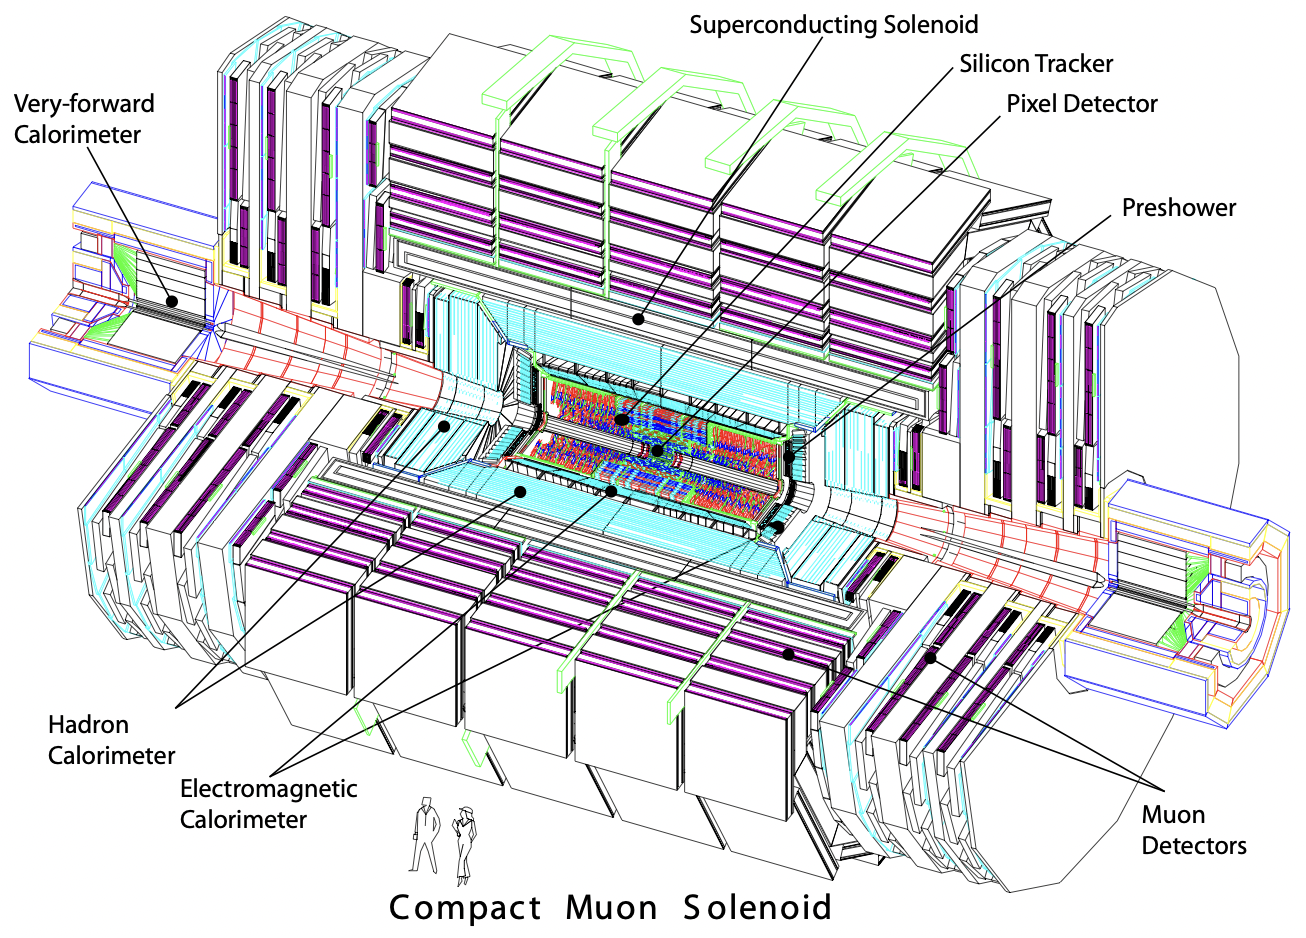
\includegraphics[width=0.6\textwidth]{figuras/CMS.png}
    \caption{A perspective view of the CMS detector \cite{CMS:2008}.}
    \label{fig:cms}
\end{figure}

\section{Data format and datasets}
\label{sec:dataset}

The CMS released reconstructed data in the CERN Open data format comes in a hierarchy of formats.
Each format sacrifices completeness for size making the choice of format the first decision required 
for an analysis using their datasets, since it fixes what information is available and what variables
are at hand. The three formats relevant here are summarised in
Table~\ref{tab:formats}.

\begin{table}[htbp]
    \centering
    \caption{The three CMS data-tier formats, in decreasing order of size and
    detail. Sizes are approximate and quoted relative to the baseline AOD.}
    \label{tab:formats}
    \begin{tabularx}{\textwidth}{@{}lXl@{}}
      \toprule
      Format & Content & Size \\
      \midrule
      AOD & High-level physics objects plus substantial lower-level
      reconstruction detail. & baseline \\[4pt]
      \midrule
      MiniAOD & Analysis-level physics objects similar to AOD but
      slimmed: many collections are reduced, extra information
      is packed into lighter objects, and less commonly used
      low-level detail is removed. &
            $\sim\!1/10$ of AOD \\[4pt]
        \midrule
      NanoAOD & Compact ntuple-style content: a limited set of per-object
      observables and precomputed IDs; little to no low-level
      detector detail (e.g., Particle Flow candidates dropped). &
            $\sim\!1/20$ of MiniAOD \\
      \bottomrule
    \end{tabularx}
\end{table}

For this work, the requirement is having access to the constituents of a jet. The substructure
observables of Chapter \ref{cap:estado-da-arte} are built by declustering a jet into its constituents,
so this analysis requires the individual particle-flow candidates that build the jet and not just 
a summary of the jet's kinematics. This immediality invalidates the NanoAOD data format since the particle-flow
candidates are not stored there. The AOD format stores the particle-flow candidates, however it also stores
other low-level reconstruction details which this analysis does not need making it occupy a large volume of
space. This leaves the MiniAOD data format, which occupies the middle ground of space and still
stores particle-flow candidates required for substructure while discarding the low-level information that is not
needed. Therefore, it is for this reason that the MiniAOD data format was the choice made for the format to be used
throughout this work.

Between all the MiniAOD datasets, this work analysed the JetHT primary dataset from the 2016 data-taking
period, in MiniAOD format~\cite{JetHT2016G}. Its characteristics are collected in
Table~\ref{tab:dataset}. The data are proton--proton collisions at a
centre-of-mass energy of $\sqrt{s} = 13$~TeV, recorded during run period G of 2016
and released as part of the Ultra-Legacy reprocessing, the final and most complete
calibration of the Run~2 data.

\begin{table}[htbp]
    \centering
    \caption{Characteristics of the JetHT primary dataset \cite{JetHT2016G}.}
    \label{tab:dataset}
    \begin{tabularx}{\textwidth}{@{}lX@{}}
      \toprule
      Property & Value \\
      \midrule
      Dataset & \texttt{/JetHT/Run2016G-UL2016\_MiniAODv2-v2/MINIAOD} \\
      Collision & proton--proton, $\sqrt{s} = 13$~TeV \\
      Run period & 2016G (runs 278820--280385) \\
      Events & $1.21 \times 10^{8}$ \\
      Size & 4.1~TiB (1236 files) \\
      \bottomrule
    \end{tabularx}
\end{table}
  
The JetHT dataset is well suited for this work analysis since it is enriched in jet events. CMS records
events online that pass a two-level trigger system, composed by a hardware Level-1 trigger followed by a software High Level Trigger
(HLT) \cite{CMS:2017trigger}. The events of this dataset are then those accepted by a set of HLT paths,
which require either a large scalar sum of jet transverse momenta
or the presence of one or two energetic jets. As a result the sample is dominated
by the high-transverse-momentum, high-multiplicity final states in which jet
substructure is most informative. Since the dataset is served by triggers based on large-radius jets, events are
required to pass one of the \texttt{HLT\_AK8PFJet} paths. The analysis is
restricted to jets with transverse momentum above $700$~GeV, where the
unprescaled paths of highest threshold, \texttt{HLT\_AK8PFJet450} and
\texttt{HLT\_AK8PFJet500}, are almost fully efficient. In this region any jet passing
the selection also satisfies these paths, so the trigger requirement introduces
no turn-on bias, and the sample sits in the hard, perturbative regime
motivated in Section~\ref{sec:qcd}.

Furthermore, as required for all analysis of this dataset, the data is restricted to a list of
runs certified as good physics, provided with the dataset release. So, events not in these
certified runs do not enter this analysis. In addition, jets in this released sample do not 
require any energy calibrations to be applied to them, since they already carry the standard jet energy corrections applied by CMS
in the Ultra-Legacy reprocessing.

Alongside the JetHT collision dataset, this analysis uses a simulated sample of QCD
multijet events. This is because the flavour of a splitting inside a jet cannot be accessed in data,
so it is not possible to determine the secondary splitting channel. What the simulation
provides is the set of generated partons, carrying flavour, which are clustered in the
same way as the reconstructed particles in data. First the partons are clustered into jets with the
anti-$\kt$ algorithm of section \ref{sec:antikt} and then, through the Cambridge/Aachen algorithm of Section
\ref{sec:ca} and the IFN algorithm of Section~\ref{sec:ifn}, into a branching
history in which each splitting acquires a flavour. It is from this process that 
the channel of each splitting, $g\to q\bar{q}$, $g\to gg$ or $q\to qg$, is labelled. 
This flavour labelling process and how it is further used in collision data is discussed in Section \ref{sec:flavour}. 
The sample used is a QCD multijet dataset generated with
\textsc{Pythia}~8~\cite{Sjostrand:2014zea} using the CP5
tune~\cite{CMS:2019csb}, passed through the full simulation of the CMS detector
and released in the same format as the collision data (MiniAODSIM)~\cite{QCDMC2016}.

\section{Analysis pipeline}
\label{sec:pipeline}

\section{Flavour selection}
\label{sec:flavour}

\section{Systematic uncertainties}
\label{sec:systematic}
\chapter{Results and Discussion}
\label{cap:resultados}

This chapter presents the results obtained from the analysis described in
Chapter \ref{cap:metodos}. They are revealed in the order in which the analysis
is built, starting by showing that the
selected jets and their substructure are described consistently in data and
simulation, followed by the results of the flavour labelling and
selection, and finally by the measurement of the spin-sensitive observables.

Section \ref{sec:res-kinematics} presents the selected jets and their kinematic
distributions. Section \ref{sec:res-lund} shows the primary and secondary Lund jet
planes, and Section \ref{sec:res-inclusive} the distribution of $\dpsi$ before any
flavour selection. Section \ref{sec:res-labelling} describes the composition of the
simulated sample in the channels defined by the IFN labelling and the modulation
associated with each of them. Section \ref{sec:res-performance} evaluates the
performance of the flavour selection and compares it with the alternative
approaches of Section \ref{sec:flavour-alternatives}. Section \ref{sec:res-modulation}
presents the central result of this work, the mean value
$\langle \cos 2\dpsi \rangle$ as a function of the threshold of the flavour
selection, in data and in simulation. Section \ref{sec:res-eeec} presents the
three-point energy correlator, and Section \ref{sec:res-discussion} discusses the
results in the light of the theoretical expectations and of the CMS measurement.

The achieved results were obtained at the level of reconstructed particles, and data
and simulation are compared at this same level. The collision data are those of the
JetHT dataset of Table~\ref{tab:dataset}, and the two simulation datasets are the
sample with $800 < \hat{p}_{\mathrm{T}} < 1000$~GeV, on which
the flavour selection is trained, and the sample with $600 < \hat{p}_{\mathrm{T}} < 800$~GeV 
which is used for the calibration of the purity
and for every comparison with data. The sample used in each figure is indicated in its
caption and, unless stated otherwise, the distributions shown are normalised to
unit area, so that their shapes are compared, and the uncertainties are
statistical only. The systematic uncertainties discussed in
Section~\ref{sec:systematic} are not represented in the figures.

\section{Event selection and jet kinematics}
\label{sec:res-kinematics}

The number of events and jets, of collision and simulation data, remaining after the selection of
Table~\ref{tab:selection} is shown in Table \ref{tab:jetcounts}. Of all the selected jets,
only those with primary and the secondary declustering contain a splitting satisfying $z > 0.1$ yield a valid
value of $\dpsi$. These jets define the sample on which all subsequent results are
based.

\begin{table}[htbp]
    \centering
    \caption{Number of events, selected jets and jets with a valid $\dpsi$, in the
    collision data and in the simulated calibration sample.}
    \label{tab:jetcounts}
    \begin{tabular}{lrrr}
      \toprule
      & Data & Simulation $600 < \hat{p}_{\mathrm{T}} < 800$ & Simulation $800 < \hat{p}_{\mathrm{T}} < 1000$ \\
      \midrule
      Events                     & 30 241 & 5 737 037 & 29 652 066 \\
      Selected jets              & 60 566 & 11 476 817 & 59 389 760 \\
      Jets with a valid $\dpsi$  & 45 755 & 8 495 207 & 43 071 113 \\
      \bottomrule
    \end{tabular}
\end{table}

The kinematic distributions of the selected jets are shown in Figure \ref{fig:jetpt},
for collision and simulation data. The three distributions start at $700$~GeV, because
of the imposed selection threshold. It is possible to see that in data, the distribution
falls smoothly and it extends to higher values, since it receives contributions from all intervals of
$\hat{p}_{\mathrm{T}}$. However, in simulation, the distributions fall much more quickly and
they struggle to reach the same higher values as in collision data, since their jets
originate from an interval of $600 < \hat{p}_{\mathrm{T}} < 800$~GeV
and $800 < \hat{p}_{\mathrm{T}} < 1000$~GeV. 
This difference is the one discussed in
Section \ref{sec:sys-purity}, and it should be kept in mind when comparing the
other distributions. Now, comparing the two simulated distribution it is worth noting that 
the $800 < \hat{p}_{\mathrm{T}} < 1000$~GeV distribution extends further above the selection threshold.
Although the flavour selection is trained, calibrated and 
applied on jets with partly different distributions, the measurement is still possible since 
the jet transverse momentum is excluded from its inputs, as discussed in
Section~\ref{sec:flavour-features}, while
the residual effect of this difference on the purity is discussed in
Section~\ref{sec:sys-purity}.

\begin{figure}[htbp]
  \centering
  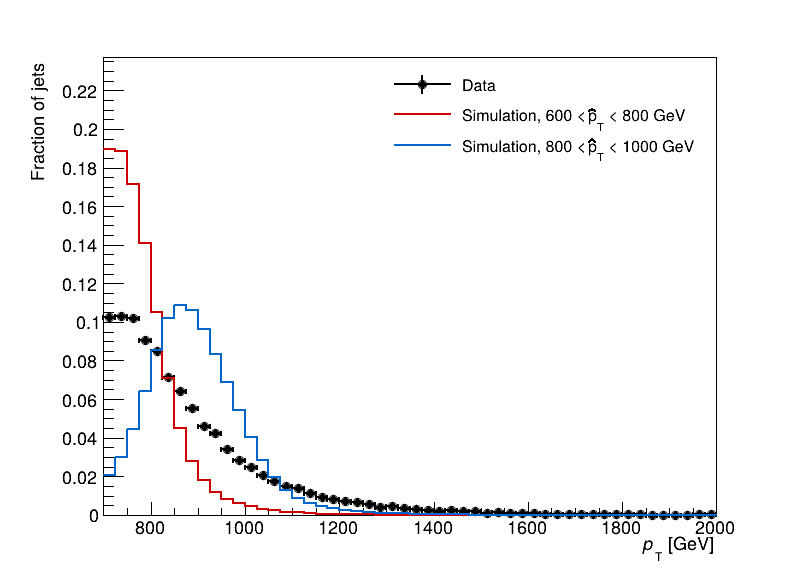
\includegraphics[width=0.6\textwidth]{figuras/jetpt_jets.png}
  \caption{Transverse-momentum distribution of the selected jets in the collision
  data and in the simulated samples with $600 < \hat{p}_{\mathrm{T}} < 800$~GeV and
  $800 < \hat{p}_{\mathrm{T}} < 1000$~GeV, normalised to unit area.}
  \label{fig:jetpt}
\end{figure}

The other distribution which is relevant for the comparison of the different
datasets is the number of constituents of the selected jets. This is the extracted
quantity most related to the substructure observables, since it shows 
the amount of radiation inside a jet, and it contributes to the flavour selection
procedure through the
multiplicities of the branches of the second splitting.
Its distribution is shown
in Figure~\ref{fig:nconst} for the collision data and for the two simulated
samples, normalised to unit area. The three distributions are very similar,
peaking at about $35$ constituents and extending up to about $130$. The simulated
samples reproduce the shape of the data very closely.

\begin{figure}[htbp]
  \centering
  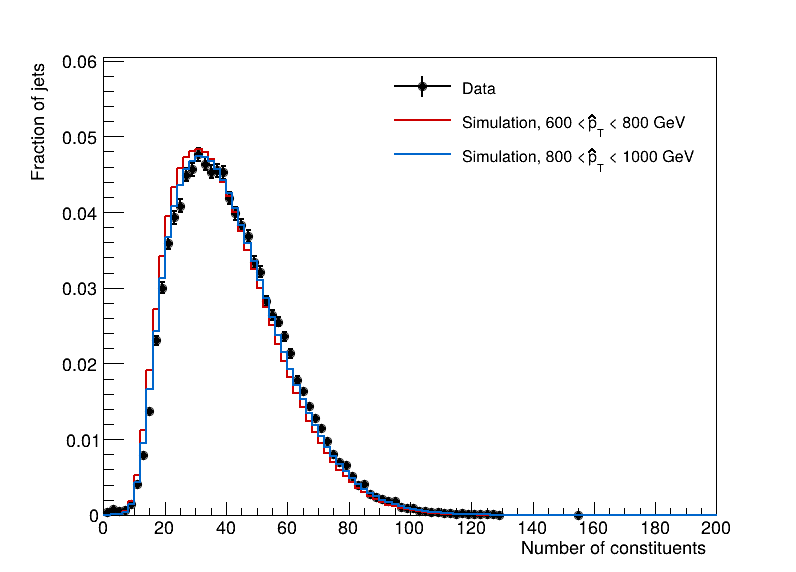
\includegraphics[width=0.6\textwidth]{figuras/nconst_jets.png}
  \caption{Number of constituents of the selected jets in the collision data and
  in the simulated samples with $600 < \hat{p}_{\mathrm{T}} < 800$~GeV and
  $800 < \hat{p}_{\mathrm{T}} < 1000$~GeV, normalised to unit area.}
  \label{fig:nconst}
\end{figure}

The very small difference between the samples represent well the pattern from their 
transverse momenta. The sample with $600 < \hat{p}_{\mathrm{T}} < 800$~GeV,
whose jets are the softest, is slightly shifted towards lower number of
constituents while the sample with $800 < \hat{p}_{\mathrm{T}} < 1000$~GeV lies closest to the
data. This difference is very small despite the very different spectra of Figure~\ref{fig:jetpt},
reflecting a slow growth of the number of constituents with the jet's transverse momentum.
The data lies slightly above both simulated samples between $50$ and $80$ constituents,
which may reflect the modelling of the
parton shower and of hadronisation, as well as differences in the pile-up
conditions between data and simulation, since neutral pile-up particles remain
among the constituents. Nevertheless, the number of constituents of the jets is 
well described by the simulation. Since the multiplicities of the branches are among the inputs of the
flavour selection, this agreement supports, although it does not by itself
establish, the transfer of the selection from simulation to data discussed in
Section~\ref{sec:sys-purity}.

\section{Lund jet planes}
\label{sec:res-lund}

The average primary and secondary Lund planes obtained from the collision and simulated calibration samples respectively,
are shown in Figure \ref{fig:lund-planes}. Each plane shows the density $\rho$ of equation \eqref{eq:lund-density},
which is the number of emissions per jet and per unit area in
the coordinates $\ln(1/\dR)$ and $\ln \kt$. Since the observable $\dpsi$ is the final measurement
of this work, only the declusterings that satisfy the condition $z > 0.1$ are included.

The shape of the populated region follows from the definition of section \ref{sec:ca}.
Since $\kt = z\,(p_{\mathrm{T},a} + p_{\mathrm{T},b})\,\dR$,
the emissions of a given branch with fixed momentum fraction lie on straight lines
of slope $-1$ in the plane,

\begin{equation}
  \ln \kt = \ln z + \ln\!\left( p_{\mathrm{T},a} + p_{\mathrm{T},b} \right)
            - \ln\frac{1}{\dR} .
  \label{eq:lund-zlines}
\end{equation}

The upper edge of the plane corresponds to the limit of $z=1/2$, because it is the largest
momentum fraction allowed when the softer branch is taken as the emission, and the
condition $z > 0.1$ imposes a parallel lower edge. Therefore, for a parent with
fixed momentum, the emissions should occupy a diagonal band of width $\ln 5$ in $\ln \kt$
at fixed angle. However, in practice, the momentum of a parent varies along the
declustering sequence and from jet to jet, which broadens the band and smooths its
edges. The left side of the plane is bounded by the radius of the jets, because the jet's 
widest splittings seperate two subjets whose axes lie within the jet, so that their
separation rarely exceeds $R = 0.8$, corresponding to $\ln(1/\dR) \approx 0.2$.

In primary Lund plane, the density along the band is approximately 
uniform at large angles and large transverse momenta, at about $0.2$ emissions per jet and per
unit area which is the expected behaviour in the perturbative region from Section \ref{sec:lund-uniform}.
In addition, towards smaller angles the density raises, reaching its maximum 
around $\ln(1/\dR) \approx 4.5$ and $\ln \kt \approx 0$, that
is for $\kt$ of order $1$~GeV, and then falling at lower transverse momenta. 
This maximum lies where $\kt$ approaches the scale of hadronisation, and marks the
transition to the non-perturbative region of the plane.

The secondary Lund plane is populated by emissions of the softer branch of the primary splitting,
but it shows the same properties. However, since this branch carries only a fraction of
momentum of the jet, the band is shifted towards lower transverse momenta, 
by about one unit in $\ln \kt$, and it is broader, as this fraction varies
from jet to jet and its maximum lies at larger angles than in the primary plane,
at around $\ln(1/\dR) \approx 3.3$. This comes from equation \eqref{eq:lund-zlines}, where
a branch with lower momentum has the region of $\kt \approx 1$~GeV, where the density peaks,
at a larger angular separation.

\begin{figure}[htbp]
  \centering
  \begin{subfigure}[b]{0.49\textwidth}
    \centering
    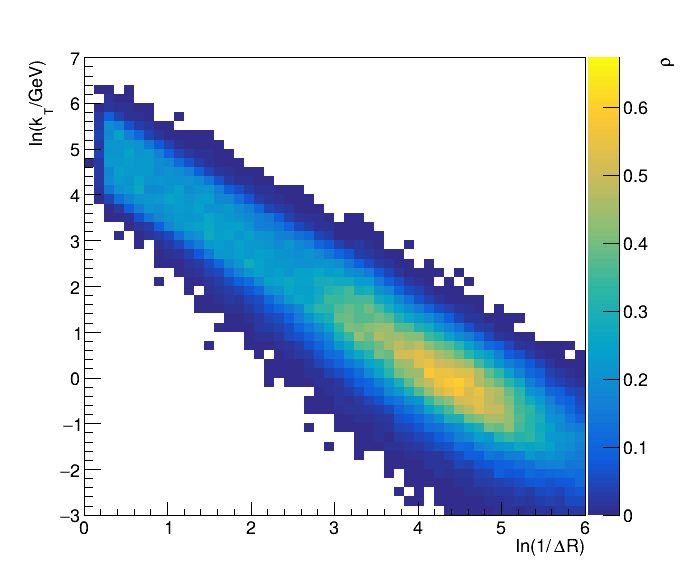
\includegraphics[width=\textwidth]{figuras/lund_primary_data.png}
    \caption{Primary plane, data.}
  \end{subfigure}
  \hfill
  \begin{subfigure}[b]{0.49\textwidth}
    \centering
    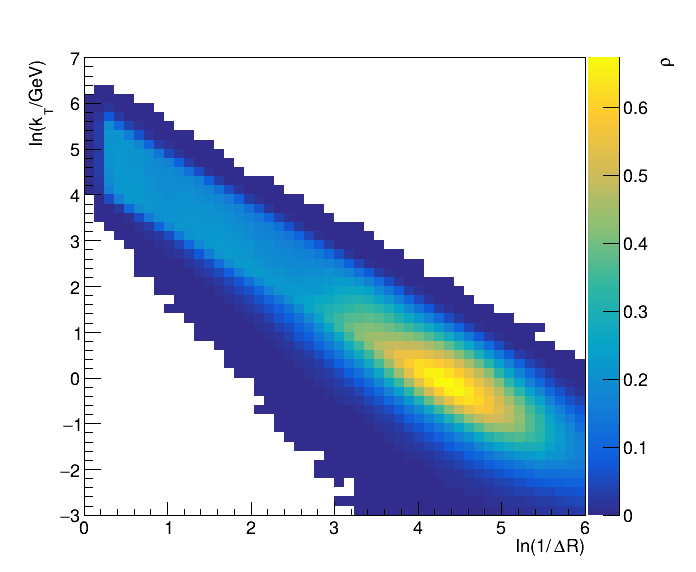
\includegraphics[width=\textwidth]{figuras/lund_primary_sim.png}
    \caption{Primary plane, simulation.}
  \end{subfigure}
  \\[6pt]
  \begin{subfigure}[b]{0.49\textwidth}
    \centering
    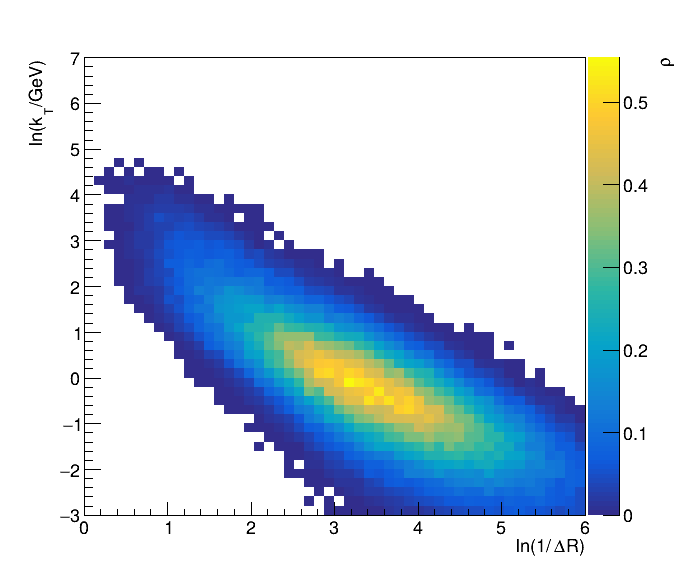
\includegraphics[width=\textwidth]{figuras/lund_secondary_data.png}
    \caption{Secondary plane, data.}
  \end{subfigure}
  \hfill
  \begin{subfigure}[b]{0.49\textwidth}
    \centering
    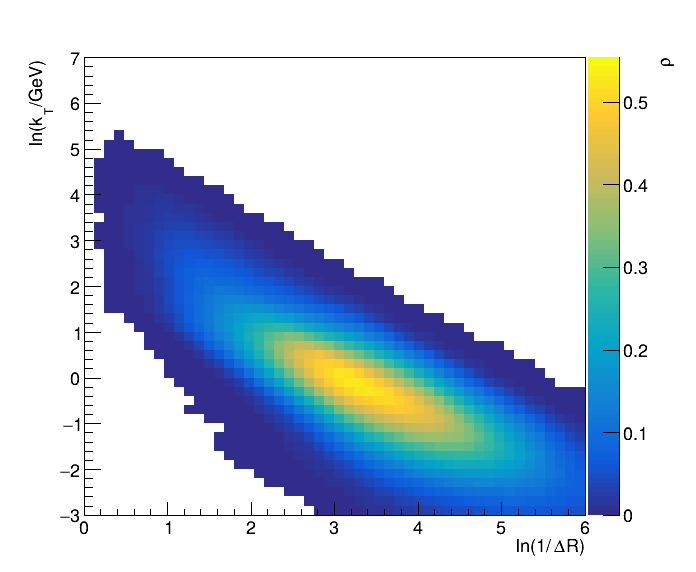
\includegraphics[width=\textwidth]{figuras/lund_secondary_sim.png}
    \caption{Secondary plane, simulation.}
  \end{subfigure}
  \caption{Average primary (top) and secondary (bottom) Lund jet planes of the jets
  with a valid $\dpsi$, in the collision data (left) and in the simulated sample
  with $600 < \hat{p}_{\mathrm{T}} < 800$~GeV (right). Only declusterings
  satisfying $z > 0.1$ are included. The colour scale shows the density of
  emissions per jet and per unit area, with the same scale for data and simulation
  in each row.}
  \label{fig:lund-planes}
\end{figure}

Now, comparing the collision data to the simulation, it is notable that they have a very close
structure. The position and
extent of the bands, and the location of their maxima, agree between data and
simulation within the precision of the maps, which
for the data show larger fluctuations owing to their smaller number of jets.
This similarity shows that the reconstruction and declustering of the jets behave
consistently in data and simulation. This also involves the quantities $z$,
$\kt$ and $\dR$ of the selected splittings, which enter the flavour selection as
inputs, and thus supports the use of the selection trained in simulation on
the collision data.

\section{Inclusive \texorpdfstring{$\dpsi$}{Delta psi 12} distribution}
\label{sec:res-inclusive}

The obtained distribution of $\dpsi$ for all jets with a valid value, before any
flavour selection, is shown in Figure \ref{fig:dpsi-inclusive} for the collision data and
for the simulated calibration sample. With the convention of equation \eqref{eq:dpsi-impl},
the angle is defined in the range of $[0,\pi]$, over which
$\cos 2\dpsi$ completes one full period. In this figure it is notable that the form of 
equation \eqref{eq:dpsi-modulation} has a negative coefficient $a_2/a_0$ with an excess 
of jets around $\dpsi = \pi/2$, where the two splitting planes are
perpendicular, and a depletion near $\dpsi = 0$ and $\pi$, where they are aligned.

\begin{figure}[htbp]
  \centering
  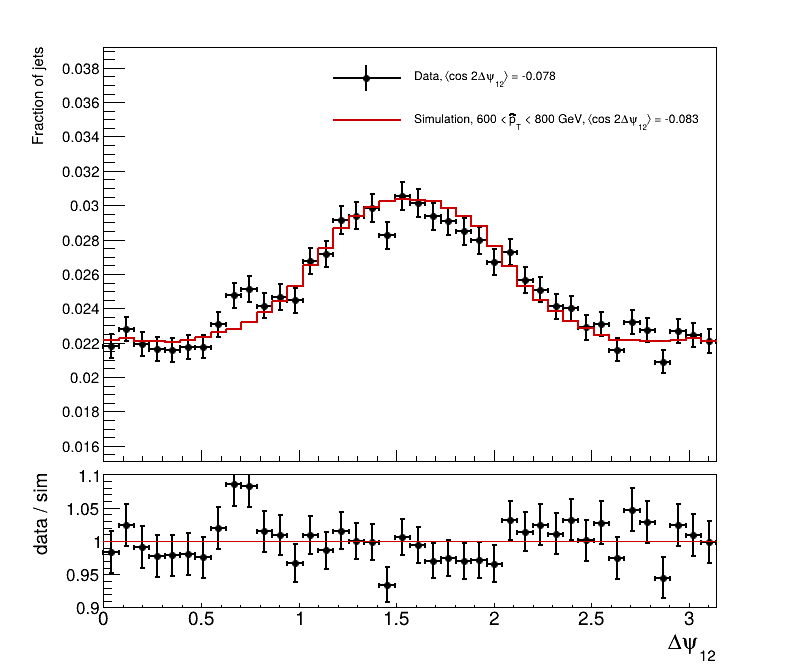
\includegraphics[width=0.7\textwidth]{figuras/dpsi_inclusive.png}
  \caption{Distribution of $\dpsi$ for all jets with a valid value, before any
  flavour selection, in the collision data and in the simulated sample with
  $600 < \hat{p}_{\mathrm{T}} < 800$~GeV, normalised to unit area.}
  \label{fig:dpsi-inclusive}
\end{figure}

The distribution shows a clear modulation of this kind. The fraction of jets rises
from about $0.022$ per bin near $\dpsi = 0$ and $\pi$ to about $0.030$ around
$\pi/2$. The mean values are

\begin{equation}
  \langle \cos 2\dpsi \rangle_{\text{data}} = -0.0780 \pm 0.0033 ,
  \qquad
  \langle \cos 2\dpsi \rangle_{\text{sim}} = -0.0831 \pm 0.0002 ,
  \label{eq:inclusive-values}
\end{equation}

where the uncertainties are statistical. Through the relation
$a_2/a_0 = 2\langle \cos 2\dpsi \rangle$, they correspond to coefficients of
$-0.156 \pm 0.007$ and $-0.166 \pm 0.001$ respectively. The two values differ by
about $1.5$ standard deviations, and the simulation describes the shape of the
distribution in data within about $5\%$ in almost every bin, the few larger
deviations being compatible with statistical fluctuations. However, the shape is not
of a pure $\cos 2\dpsi$ modulation since the distribution is nearly flat close to 
$\dpsi = 0$ and $\pi$, and its central maximum is narrower than of a single harmonic modulation, 
which may indicate the presence of higher harmonics in addition to the
$\cos 2\dpsi$ term.

This inclusive result is dominated by splittings that are unmatched or belong to channels
other than $g \to q\bar{q}$, as shown in Table~\ref{tab:composition}. Therefore, this modulation
is a superposition of all contributions of different channels and it is diluted according to it.
Thus, this distribution serves as baseline for evaluating the impact of the flavour selection 
in Section~\ref{sec:res-performance}, while the significance of its magnitude is examined in Section~\ref{sec:res-modulation}.

\section{Channel labelling}
\label{sec:res-labelling}

The composition of the simulated training sample in the channels defined by the
IFN labelling of Section~\ref{sec:genlevel} is given in
Table~\ref{tab:composition} while for the simulated calibration sample is given by
the following Table~\ref{tab:cos2-labels}. The composition obtained also agrees closely with 
the one obtained in the
CMS measurement with \textsc{Pythia}~8, the same flavour definition and the same
matching of the branches $p_3$ and $p_4$, namely $72\%$, $16\%$, $8\%$, $3\%$ and
$1\%$~\cite{CMS:2026jnt}. The agreement confirms that the labelling was constructed 
correctly, although it does not prove whether the
simulation describes the data.

The mean value $\langle \cos 2\dpsi \rangle$ obtained from the simulated 
calibration sample is also given in Table~\ref{tab:cos2-labels},
together with the value predicted at second
order in the collinear limit for the corresponding channel~\cite{Karlberg_2021}.
This prediction was computed on electron-positron collisions without hadronisation
or detector effects, and, in this work, it serves only as a reference point for the sign 
and the order of magnitude of each contribution

\begin{table}[htbp]
  \centering
  \caption{Mean value $\langle \cos 2\dpsi \rangle$ for the jets of each channel of
  the IFN labelling, in the simulated calibration sample, with statistical
  uncertainties. The last column gives the prediction of
  Ref.~\cite{Karlberg_2021} for the corresponding channel, obtained for
  electron-positron collisions with $z_1, z_2 > 0.1$.}
  \label{tab:cos2-labels}
  \begin{tabular}{lrrrr}
    \toprule
    Class & Jets & Fraction (\%) & $\langle \cos 2\dpsi \rangle$ & Prediction \\
    \midrule
    $g \to q\bar{q}$   & $179\,810$     & $3.1\%$  & $-0.167 \pm 0.002$ & $-0.31$ \\
    $g \to gg$         & $857\,140$     & $14.7\%$ & $-0.077 \pm 0.001$ & $+0.025$ \\
    $q \to qg$         & $358\,498$     & $6.1\%$  & $-0.091 \pm 0.001$ & $0$ \\
    unmatched          & $4\,397\,983$  & $75.2\%$ & $-0.0585 \pm 0.0003$ & --- \\
    rest               & $53\,911$      & $0.9\%$  & $-0.161 \pm 0.003$ & --- \\
    \midrule
    all labelled jets  & $5\,847\,342$  & $100\%$ & $-0.0674 \pm 0.0003$ & ---\\
    \bottomrule
  \end{tabular}
\end{table}

The $g \to q\bar{q}$ channel shows a modulation with $\langle \cos 2\dpsi \rangle = -0.167 \pm 0.002$,
while the $q \to qg$ and $g \to gg$ channels, which form the background of the flavour selection, give
together $-0.081 \pm 0.001$. Thus, the modulation of the $g \to q\bar{q}$ channel is
about twice as strong as that of the background, and it is this
difference that the flavour selection exploits. In Figure~\ref{fig:qq_vs_all}, it is possible to see
the difference between the $g \to q\bar{q}$ channel and the whole sample. It is important 
to note that the sign of the $g \to q\bar{q}$ class agrees with the prediction, while its magnitude
is smaller which is expected for a flavour based label that does not coincide splitting by splitting with the channel
of the parton shower and for an observable built from reconstructed particles. More importantly,
the $q \to qg$ and $g \to gg$ classes also show a negative sign in contrast with 
the vanishing and slightly positive values predicted for the
corresponding channels. A negative contribution is thus present in every class,
including those in which no spin correlation is expected and its source is discussed
in Section~\ref{sec:res-discussion}.

\begin{figure}[htbp]
  \centering
  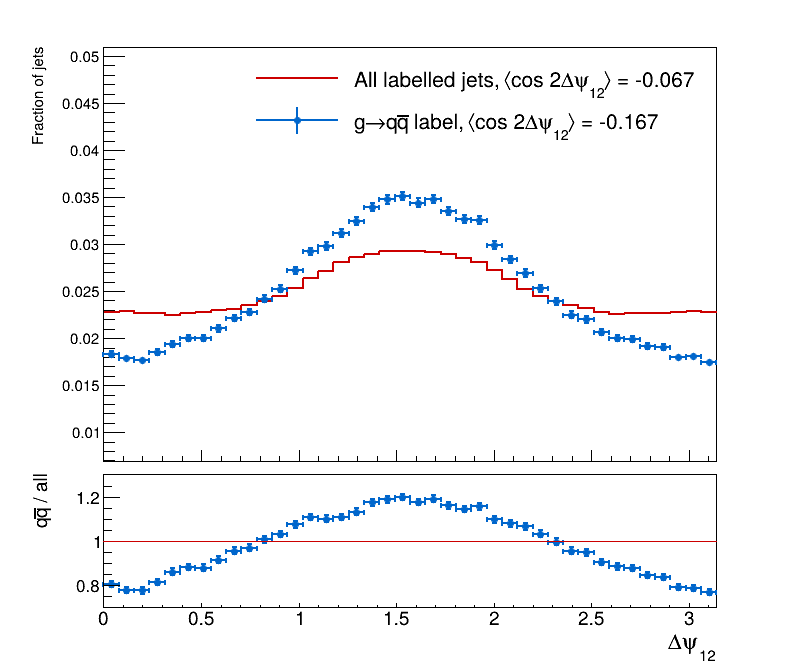
\includegraphics[width=0.7\textwidth]{figuras/dpsi_labels.png}
  \caption{Distribution of $\dpsi$ for all labelled jets and for the jets whose
  second splitting is labelled $g \to q\bar{q}$, in the simulated sample with
  $600 < \hat{p}_{\mathrm{T}} < 800$~GeV, normalised to unit area. The lower
  panel shows the ratio of the $g \to q\bar{q}$ distribution to that of all
  labelled jets.}
  \label{fig:qq_vs_all}
\end{figure}

\subsection{Momentum fractions of the two splittings}
\label{sec:res-zplane}

The momentum fractions $z_1$ and $z_2$ of the primary and secondary selected splittings
are two of the features used by the flavour selection of
Section~\ref{sec:flavour}. Each is the fraction carried by the softer branch and lies
between the SoftDrop grooming condition of $z = 0.1$ and $z = 1/2$. Their complete
distribution is shown in Figure \ref{fig:zplane-channels} for all jets with a valid 
$\dpsi$, in data and in simulation, and for the simulated jets in each channel.
The ratio of each distribution to that of all simulated jets is shown in
Figure~\ref{fig:zplane-ratios}, where the differences between the channels can be 
distinguished more easily.

\begin{figure}[htbp]
  \centering
  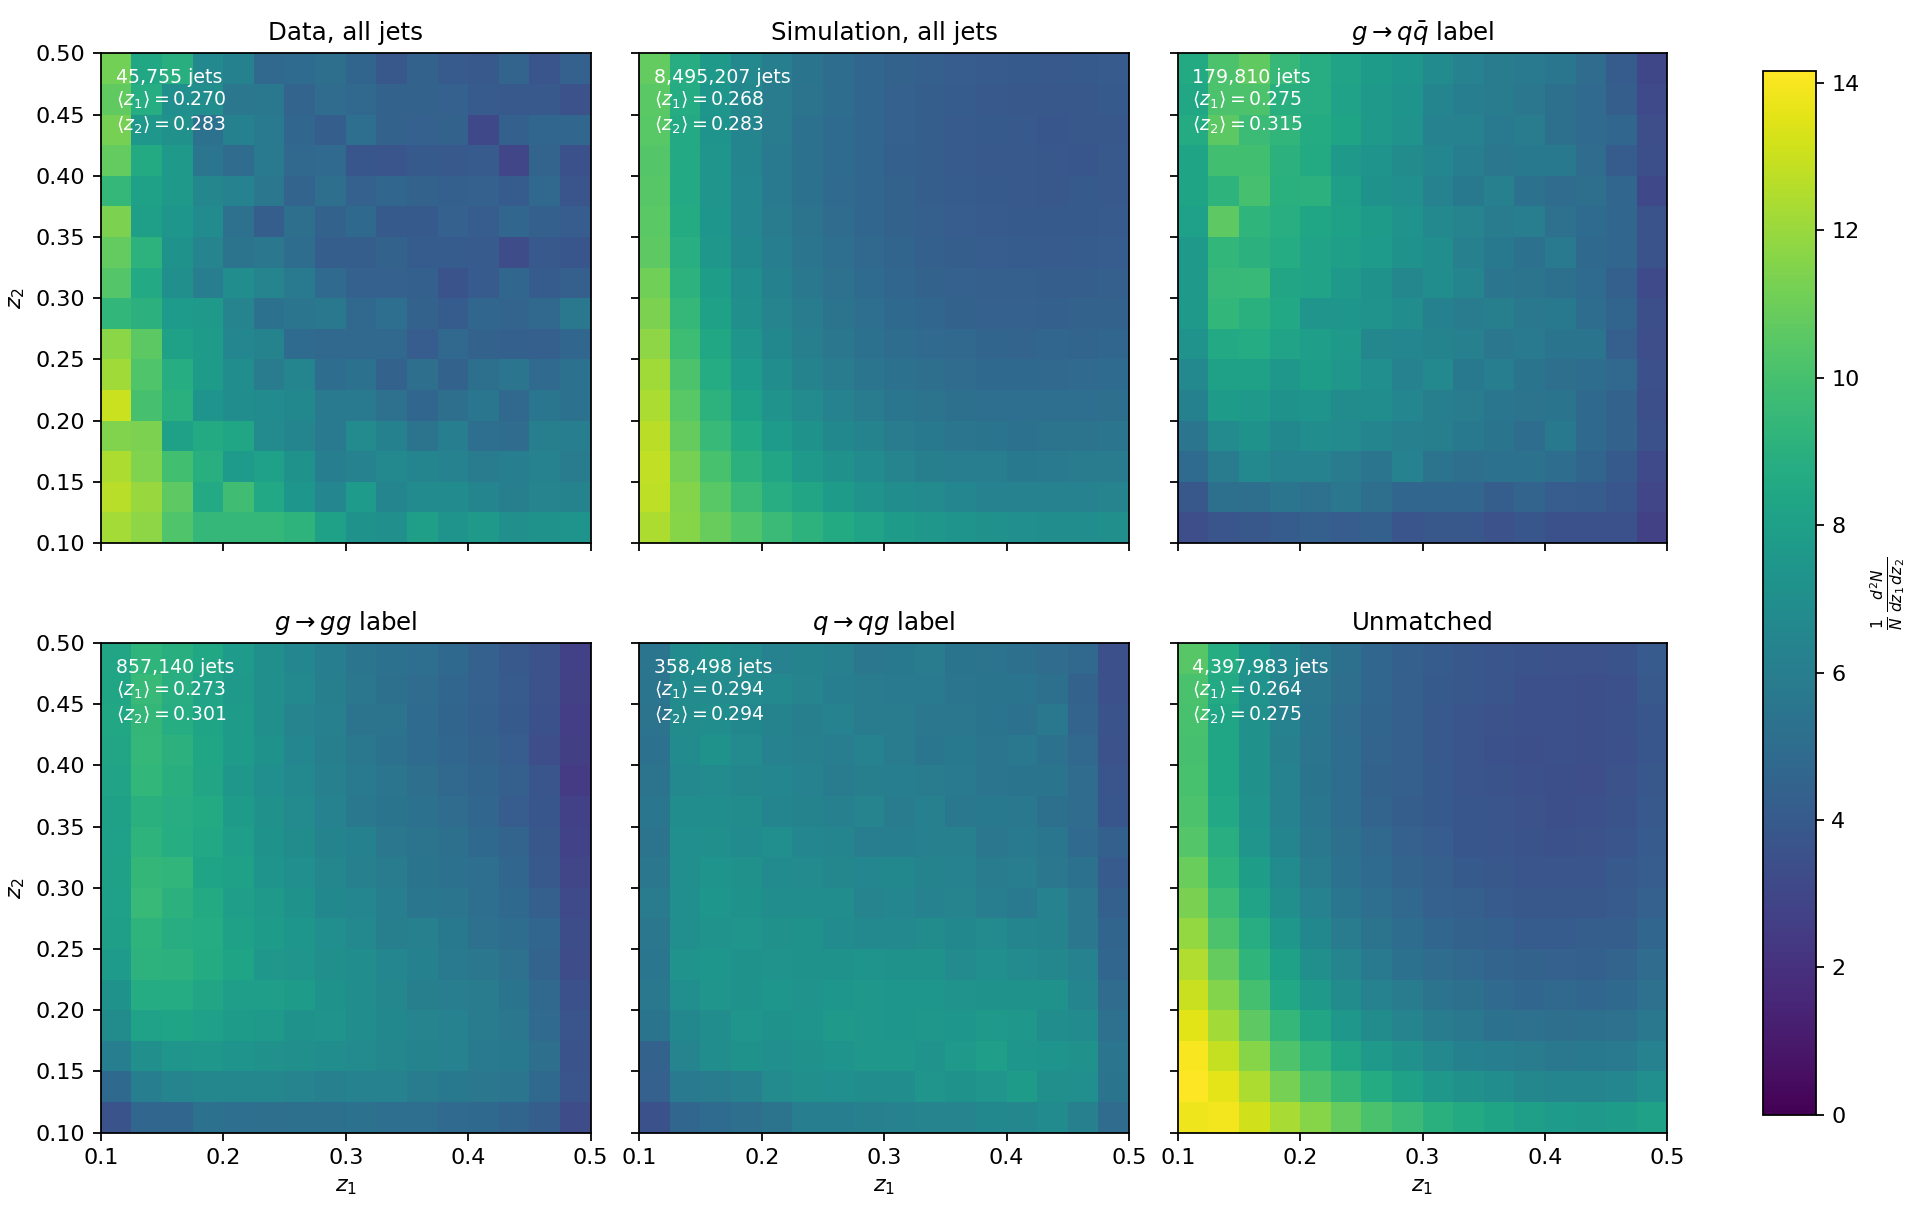
\includegraphics[width=\textwidth]{figuras/zplane_channels.png}
  \caption{Distribution of the momentum fractions $z_1$ and $z_2$ of the first and
  second selected splittings, normalised to unit area, for all jets with a valid
  $\dpsi$ in the collision data and in the simulated calibration sample, and for
  the simulated jets labelled $g \to q\bar{q}$, $g \to gg$ and $q \to qg$ and
  those unmatched. Each panel gives the number of jets and the mean values of
  $z_1$ and $z_2$.}
  \label{fig:zplane-channels}
\end{figure}

\begin{figure}[htbp]
  \centering
  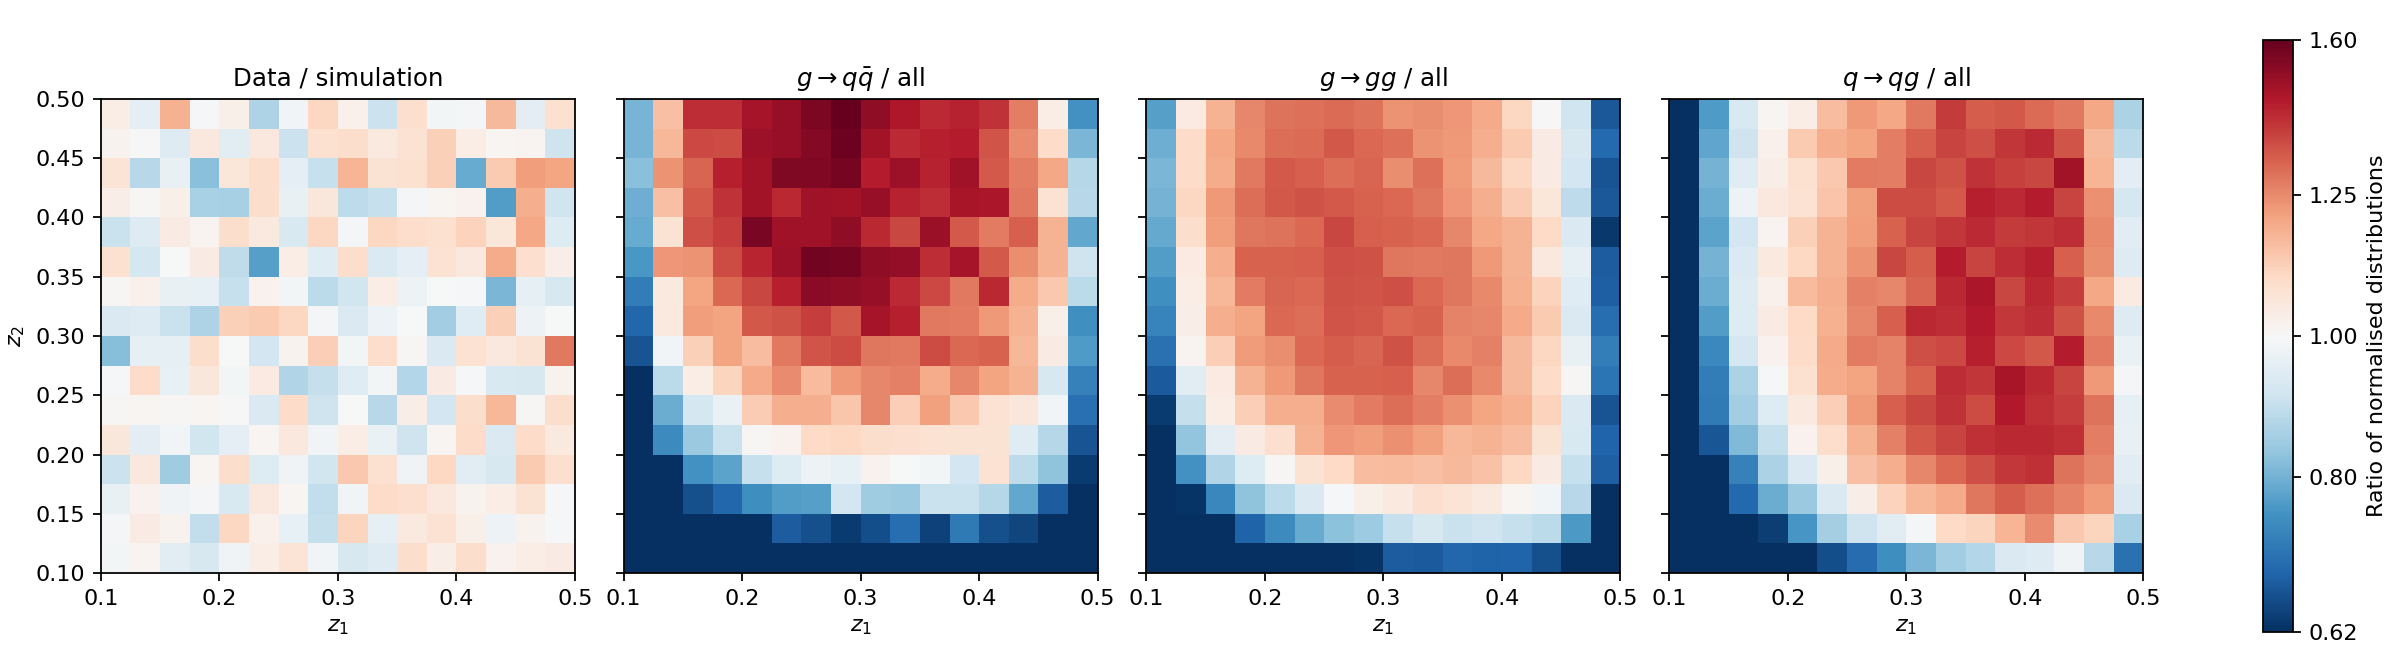
\includegraphics[width=\textwidth]{figuras/zplane_ratios.png}
  \caption{Ratio of the normalised distributions of
  Figure~\ref{fig:zplane-channels} to that of all simulated jets, for the
  collision data and for the simulated jets labelled $g \to q\bar{q}$, $g \to gg$
  and $q \to qg$. The colour scale is logarithmic and symmetric around unity, and
  ratios beyond its range are shown at its limits.}
  \label{fig:zplane-ratios}
\end{figure}

The distribution of all jets is concentrated at small $z_1$ and $z_2$, so that asymmetric splittings
with soft branch dominate the sample. The simulation describes the collision data well
with mean values of $\langle z_1 \rangle = 0.270$ and $\langle z_2 \rangle = 0.283$ in data, against
$0.268$ and $0.283$ in simulation, and the ratio of the two distributions shows no
systematic structure, only fluctuations compatible with the statistical
precision of the data.

The channels populate the plane differently. The unmatched jets, which make up
about half of the sample, are concentrated in the corner of small $z_1$ and $z_2$,
with $\langle z_1 \rangle = 0.264$ and $\langle z_2 \rangle = 0.275$. Soft branches
are the most affected by hadronisation and by the detector, so their splittings
are the least often matched at generator level. The labelled channels instead
populate the interior of the plane. The jets labelled $g \to q\bar{q}$ have the
largest $\langle z_2 \rangle$, $0.315$. Relative to all jets they are enhanced by
$50\%$ or more for $0.3 \lesssim z_2 \lesssim 0.45$ and intermediate $z_1$, and
suppressed by more than a third for $z_2 < 0.15$. This reflects the splitting
function of Eq.~\eqref{eq:Pgq}, which has no enhancement for soft splittings,
in contrast with those of $g \to gg$ and $q \to qg$. The jets labelled $g \to gg$
show a similar but weaker pattern, with $\langle z_2 \rangle = 0.301$. The jets
labelled $q \to qg$ differ mainly in $z_1$, with the largest mean value,
$\langle z_1 \rangle = 0.294$, and an enhancement at $z_1 \gtrsim 0.3$.
For the second splitting to be $q \to qg$, the softer branch of the first splitting must
be a quark, and a quark is produced without the soft enhancement associated with
an emitted gluon. Therefore, the first splitting of these jets is more symmetric.

As one can notice, all channels have a depletion near the edge of $z_1 \to 1/2$.
When the primary splitting is nearly symmetric, its softer branch is decided by small
differences in the transverse momentum of the splitting's daughters. So, 
the generator-level and the reconstructed declusterings can then follow different
branches to the secondary splitting, making the algorithm label the secondary 
splitting as unmatched.

These differences are the information in $z_1$ and $z_2$ that the flavour
selection can exploit. The $g \to q\bar{q}$ channel is distinguished mainly by
its more symmetric second splitting, and the effect of the selection on the
distribution of $z_2$ is examined in Section~\ref{sec:res-mod-z}.

\section{Flavour selection performance}
\label{sec:res-performance}

In order to measure the spin-sensitive observable using the flavour selection, discussed
in Section \ref{sec:flavour}, it must first be shown that it can identify the $g \to q\bar{q}$ channel
effectively. This section evaluates its performance in simulation, where the IFN
label of every splitting is known, and compares it with the alternative approaches
of Section~\ref{sec:flavour-alternatives}.

As stated before, two simulated samples were used, for different purposes. 
The separation achieved by
each network is assessed on the test subset of the training sample, with
$800 < \hat{p}_{\mathrm{T}} < 1000$~GeV, which was not used during the training.
It is characterised by the distributions of the scores for the different channels
and by the area under the ROC curve, which measures the ability of the network to
rank a splitting of the signal channels above one of the background. For the second
stage, in which the $g \to q\bar{q}$ channel is a minority, the area under the
precision-recall curve is also given, since it reflects more directly the purity
that can be achieved. The performance of the complete selection, expressed through
the purity and the efficiency of equation \eqref{eq:purity-efficiency}, is determined
instead on the independent calibration sample, with
$600 < \hat{p}_{\mathrm{T}} < 800$~GeV. This is the sample on which the purity of
the measurement is calibrated, and it allows all methods to be compared without
any bias from their training.

Section~\ref{sec:res-twostage} presents the performance of the two stages of the
selection and the purity reached as a function of the threshold.
Section~\ref{sec:res-alternatives} compares the two-stage selection with the
alternative approaches.

\subsection{Two-stage selection}
\label{sec:res-twostage}

The first stage network separates matched from unmatched splittings performing it with an area
under the ROC curve of $0.840$, as shown in Figure~\ref{fig:roc-stage1}. This network 
performance is sufficient in order to remove the majority number of unmatched secondary
splittings before the flavour of the second splitting is examined. In Figure~\ref{fig:confusion},
the confusion matrix of the first stage classifier, obtained from the test subset, is shown.
Since unmatched splittings form the bulk of the data sample, a classifier trained on this imbalance
could assign almost all splittings to this class. The matrix presented reveals that this is 
not the case. The results revealed that of the unmatched splittings, $87.4\%$ are correctly identified and $12.6\%$ are
classified as matched, while $61.8\%$ of the matched splittings are correctly
identified and $38.2\%$ are classified as unmatched. Therefore, both classes were
recognised as intended by the class weights during training. However, since the
unmatched splittings are about three times more numerous, the $12.6\%$
of them classified as matched still make up about $40\%$ of all the splittings
assigned to the matched class. This is why the matched score is set to be above
$0.8$, rather than the assignment to the most probable class on which the matrix is based.

\begin{figure}[htbp]
  \centering
  \begin{subfigure}[b]{0.49\textwidth}
    \centering
    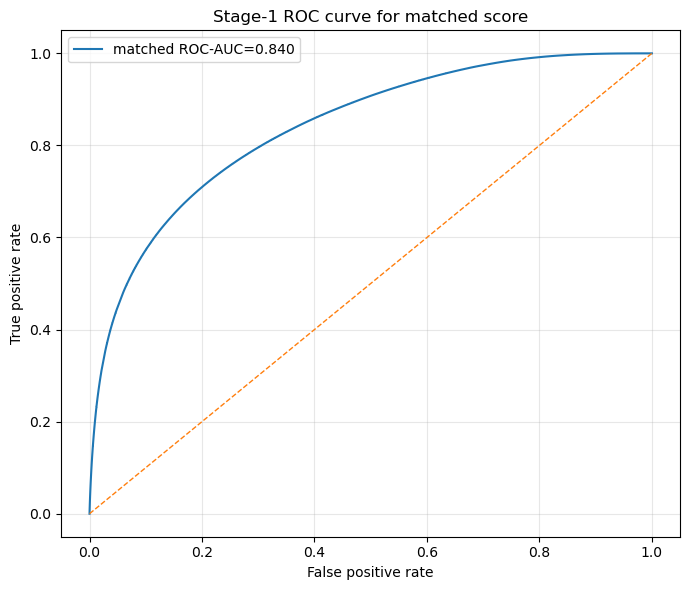
\includegraphics[width=\textwidth]{figuras/roc_stage1.png}
    \caption{ROC curve.}
    \label{fig:roc-stage1}
  \end{subfigure}
  \hfill
  \begin{subfigure}[b]{0.49\textwidth}
    \centering
    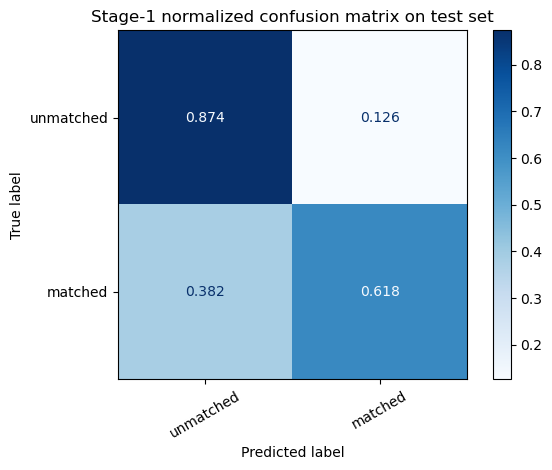
\includegraphics[width=\textwidth]{figuras/confusion.png}
    \caption{Confusion matrix.}
    \label{fig:confusion}
  \end{subfigure}
  \caption{Performance of the first stage on the test subset of the simulated
  sample with $800 < \hat{p}_{\mathrm{T}} < 1000$~GeV. (a) ROC curve of the matched
  score. (b) Confusion matrix, in which each row is normalised to the number of
  splittings of the corresponding true class and each splitting is assigned to
  the class of highest probability.}
  \label{fig:stage1-performance}
\end{figure}

The performance of the second stage is evaluated on the population 
on which it was trained which are the splittings labelled as $g \to q\bar{q}$, $q \to qg$ or $g \to gg$.
The distribution of its score for the $g \to q\bar{q}$ class and for the other two
classes together is shown in Figure~\ref{fig:score-stage2}. Both distributions
peak at about $0.3$, and the background is concentrated in the range between $0.2$ and $0.4$.
The main and most important difference between these two distributions is that the 
$g \to q\bar{q}$ class has a long tail extending to scores of about $0.65$, in which it dominates.
These scores are although confined between $0.15$ and $0.7$, which reflects the strong overlap
of the channels in the space of the input features and the use of the focal loss,
which does not push the outputs towards the extreme values.

\begin{figure}[htbp]
  \centering
  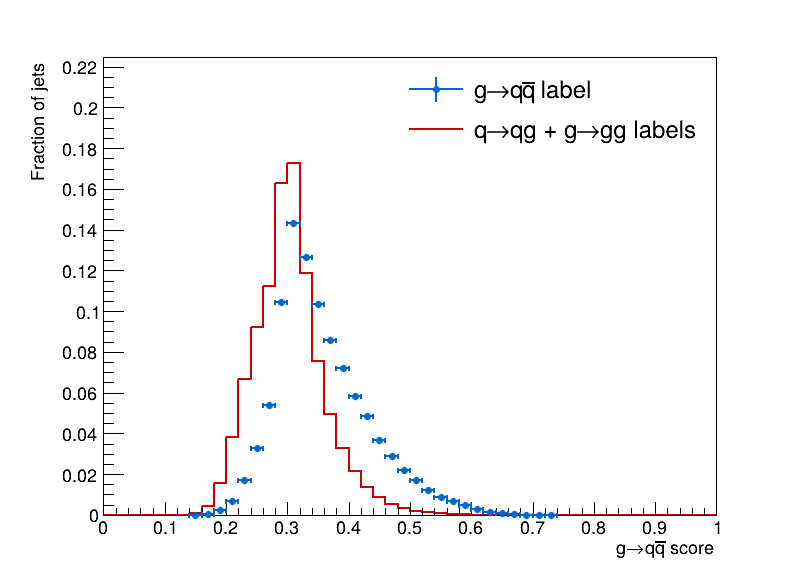
\includegraphics[width=0.7\textwidth]{figuras/score_stage2.png}
  \caption{Distribution of the $g \to q\bar{q}$ score of the second stage for the
  $g \to q\bar{q}$ class and for the $q \to qg$ and $g \to gg$ classes together, on
  the simulated calibration sample with $600 < \hat{p}_{\mathrm{T}} < 800$~GeV,
  normalised to unit area.}
  \label{fig:score-stage2}
\end{figure}

The ROC and precision-recall curves are shown in Figure~\ref{fig:roc-pr-stage2}.
The area under the ROC curve is $0.714$, which is worse compared to the first stage classifier, and the
area under the precision-recall curve is $0.314$, compared with $0.129$ for a
classifier without discriminating power, which corresponds to the fraction of the
$g \to q\bar{q}$ class among the matched splittings. The same areas were computed 
on the simulated calibration sample and the values of $0.715$ and $0.314$ were obtained for the 
ROC and precision-recall curves respectively. These values show that this network generalises 
to jets outside its training sample and the precision-recall curve also shows 
that a high purity is reached only at a small
efficiency, the purity exceeding $0.6$ only for efficiencies below about $10\%$.

\begin{figure}[htbp]
  \centering
  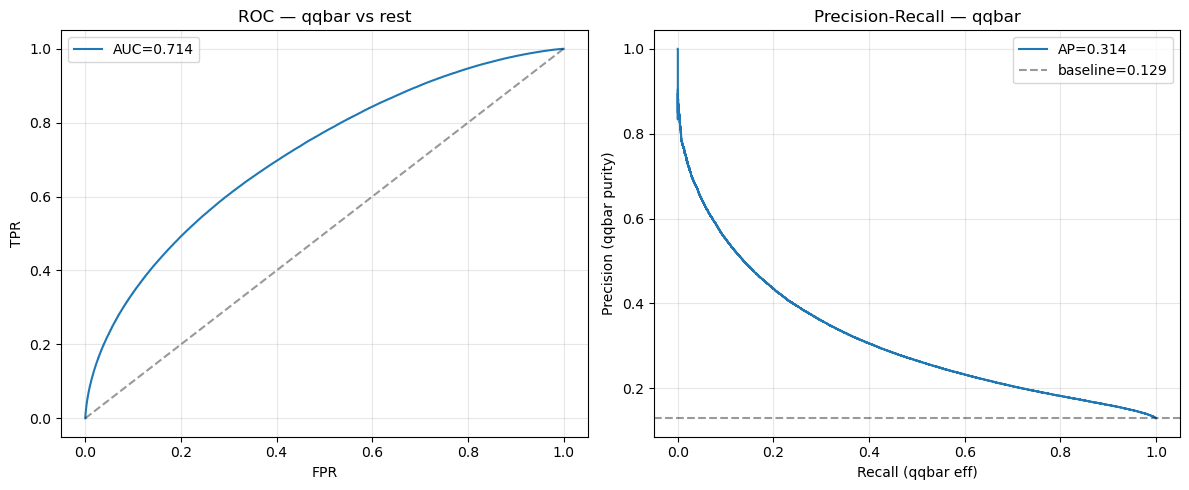
\includegraphics[width=\textwidth]{figuras/roc_pr_stage2.png}
  \caption{ROC curve (left) and precision-recall curve (right) of the
  $g \to q\bar{q}$ score of the second stage. The dashed line in the right panel
  shows the precision of a classifier without discriminating power.}
  \label{fig:roc-pr-stage2}
\end{figure}

The purity and the efficiency of the second stage on the test sample are
given in Table~\ref{tab:purity-threshold} and shown in
Figure~\ref{fig:purity-efficiency-threshold} as a function of the threshold.
As the threshold increases from $0.30$ to $0.60$, the purity rises steadily from
$0.18$ to $0.80$, while the efficiency falls from $81\%$ to below $1\%$. Above
$0.60$ the purity continues to rise, but the number of selected jets falls to a
few hundred and then even less, meaning that these thresholds carry little statistical
weight.

\begin{table}[htbp]
  \centering
  \caption{Number of selected jets, purity and efficiency of the second stage as a
  function of the threshold on the $g \to q\bar{q}$ score, for the splittings
  labelled $g \to q\bar{q}$, $q \to qg$ or $g \to gg$ in the simulated calibration
  sample with $600 < \hat{p}_{\mathrm{T}} < 800$~GeV. The uncertainties on the
  purity are statistical, and the efficiency is relative to all splittings
  labelled $g \to q\bar{q}$.}
  \label{tab:purity-threshold}
  \begin{tabular}{rrcr}
    \toprule
    Threshold & Selected jets & Purity & Efficiency (\%) \\
    \midrule
    $0.30$ & $1\,319\,798$ & $0.1807 \pm 0.0003$ & $80.6$ \\
    $0.35$ & $534\,802$    & $0.270 \pm 0.001$ & $48.7$ \\
    $0.40$ & $211\,459$    & $0.379 \pm 0.001$ & $27.1$ \\
    $0.45$ & $81\,911$     & $0.500 \pm 0.002$ & $13.8$ \\
    $0.50$ & $30\,446$     & $0.616 \pm 0.003$ & $6.3$ \\
    $0.55$ & $10\,111$     & $0.716 \pm 0.005$ & $2.5$ \\
    $0.60$ & $2\,455$      & $0.802 \pm 0.008$ & $0.67$ \\
    $0.65$ & $319$         & $0.865 \pm 0.019$ & $0.09$ \\
    $0.70$ & $16$          & $0.94 \pm 0.06$   & $0.01$ \\
    \bottomrule
  \end{tabular}
\end{table}

\begin{figure}[htbp]
  \centering
  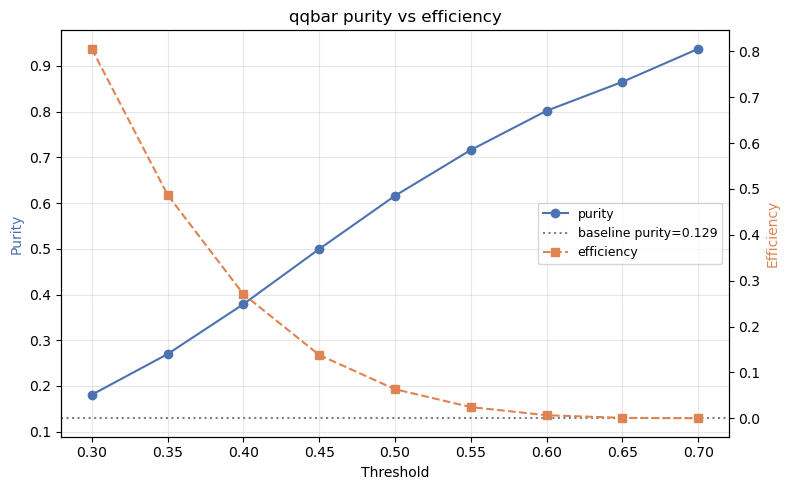
\includegraphics[width=0.75\textwidth]{figuras/purity_efficiency.png}
  \caption{Purity (left axis) and efficiency (right axis) of the second stage as a
  function of the threshold on the $g \to q\bar{q}$ score, for the splittings
  labelled $g \to q\bar{q}$, $q \to qg$ or $g \to gg$ in the simulated calibration
  sample. The dotted line shows the fraction of $g \to q\bar{q}$ splittings among
  these, before any selection.}
  \label{fig:purity-efficiency-threshold}
\end{figure}

\subsection{Comparison with alternative approaches}
\label{sec:res-alternatives}

The three alternative approaches of Section~\ref{sec:flavour-alternatives} are compared with the
previous two-stage selection on the simulated calibration sample. A first comparison
was made regarding the performance of the networks, evaluated on the splittings labelled as
$g \to q\bar{q}$, $q \to qg$ or $g \to gg$. On this population, the areas under the
ROC and precision--recall curves are $0.715$ and $0.314$ for the second stage of
the two-stage selection, $0.710$ and $0.309$ for the three-class network, and
$0.693$ and $0.300$ for the four-class network. Thus, the three different networks reach
a very similar performance, meaning that the selection of the $g \to q\bar{q}$ channel
is limited by the input features rather than the architecture of the network. 
The Gaussian
mixture model provides no useful separation, the purities of its clusters lying
between about $0.10$ and $0.16$, close to the fraction of $g \to q\bar{q}$
splittings among the matched ones.

However, this first comparison totally ignores the unmatched splittings, which the
four-class network rejects at the same time as it identifies the
$g \to q\bar{q}$ channel. The more relevant comparison for the measurement
of this work is that of the complete selections, applied to all labelled splittings.
The two-stage selection requires a matched score above $0.8$ and a threshold on the
second-stage score. The second selection replaces the second stage by the
three-class network after the same requirement on the matched score. The third
applies a threshold on the output of the four-class network alone.
Thus the purity of each selection, including the unmatched splittings among the selected jets,
are shown in Figure~\ref{fig:purity-full} as a function of its efficiency, and its
value at different efficiencies is given in Table~\ref{tab:purity-full}.

\begin{figure}[htbp]
  \centering
  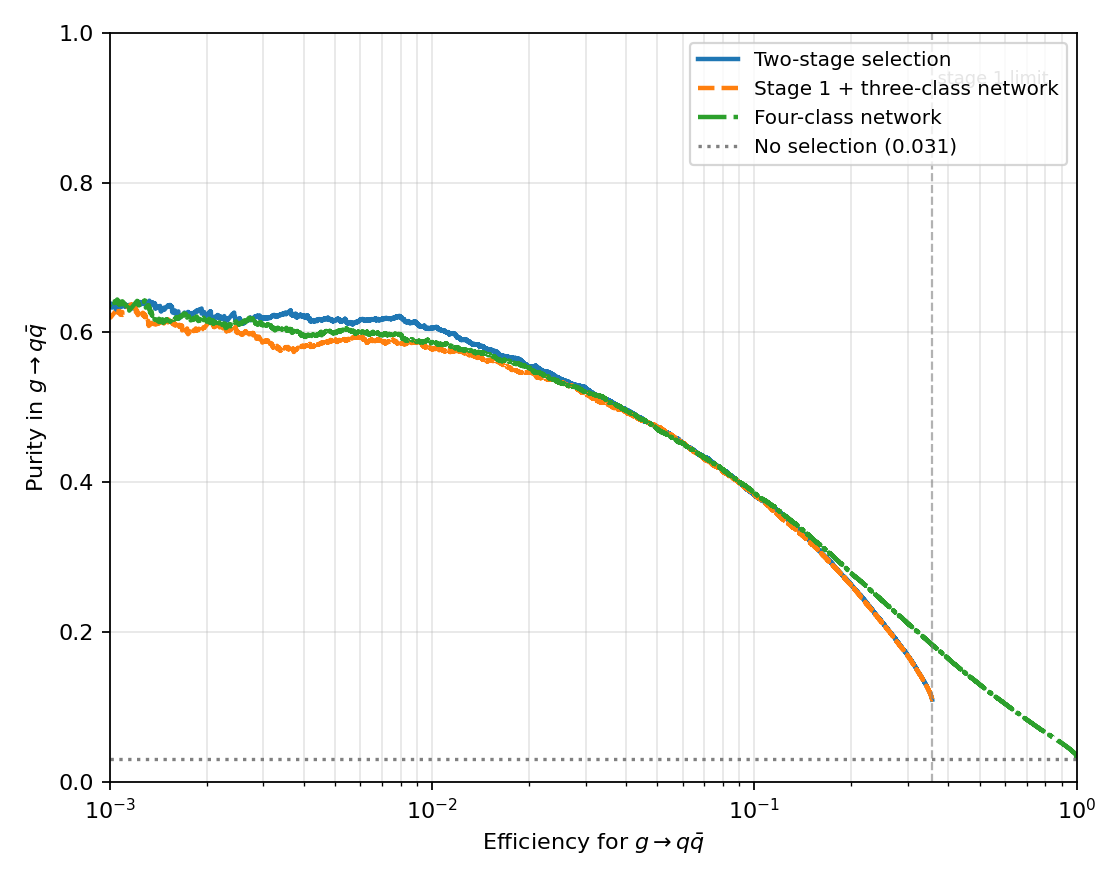
\includegraphics[width=0.75\textwidth]{figuras/purity_full_methods.png}
  \caption{Purity as a function of efficiency for the $g \to q\bar{q}$ channel,
  for the complete two-stage selection, for the first stage followed by the
  three-class network, and for the four-class network, applied to all labelled
  splittings of the simulated calibration sample. The vertical line marks the
  largest efficiency allowed by the requirement on the matched score, and the
  dotted line the purity before any selection.}
  \label{fig:purity-full}
\end{figure}

\begin{table}[htbp]
  \centering
  \caption{Purity of the complete selections at fixed efficiencies for the
  $g \to q\bar{q}$ channel, on all labelled splittings of the simulated
  calibration sample.}
  \label{tab:purity-full}
  \begin{tabular}{rccc}
    \toprule
    Efficiency (\%) & Two-stage & Stage 1 + three-class & Four-class \\
    \midrule
    $0.5$ & $0.622$ & $0.595$ & $0.606$ \\
    $1$   & $0.608$ & $0.579$ & $0.587$ \\
    $2$   & $0.556$ & $0.547$ & $0.553$ \\
    $5$   & $0.474$ & $0.475$ & $0.471$ \\
    $10$  & $0.383$ & $0.384$ & $0.386$ \\
    $20$  & $0.263$ & $0.262$ & $0.279$ \\
    $30$  & $0.168$ & $0.168$ & $0.211$ \\
    \bottomrule
  \end{tabular}
\end{table}

The three selections behave differently in different regions. At efficiencies
below about $2\%$, where the purity is highest, the two-stage selection reaches the
largest purity, by about $0.02$ to $0.03$ at an efficiency of $1\%$, a difference
of two to three times the statistical uncertainty of the purity. Between $5\%$ and
$10\%$ the three selections are equivalent. At larger efficiencies the four-class
network performs better, and it alone can exceed the efficiency of $35.7\%$ to
which the requirement on the matched score limits the other two. This is the
advantage of treating the rejection of the unmatched splittings and the
identification of the $g \to q\bar{q}$ channel in a single step.

However, for this measurement, the region of interest is the one with the highest purity
possible while keeping enough statistics. The
thresholds used in Section~\ref{sec:res-modulation} correspond to efficiencies
between about $28\%$ and $0.5\%$, and the most enriched samples lie below $5\%$,
where the two-stage selection performs best. The
two-stage selection is therefore retained for the measurement.

\section{Spin modulation as a function of the flavour selection}
\label{sec:res-modulation}

Finally, this section presents the main result of this work, the mean value
$\langle \cos 2\dpsi \rangle$ of the jets selected by the two-stage selection, as a
function of the threshold on the $g \to q\bar{q}$ score. Again, every jet is required 
to have a matched score greater than $0.8$ and the threshold on the second score goes
from $0.30$ to $0.60$ in steps of $0.05$. Because of statistics, the function does not
continue past $0.60$, since the number of selected jets becomes too small 
for the mean value to carry useful information, as discussed in
Section~\ref{sec:flavour-application}. Each threshold defines a sample increasingly
enriched in the $g \to q\bar{q}$ channel, and the evolution of the modulation along
this sequence of samples is the quantity of interest.

The purity computed for each threshold is that of a complete selection, determined 
in the simulation calibration sample. Its value depends on the treatment
of the jets that carry no channel label, for which no generator-level counterpart
was found or the generator-level declustering failed. These jets make up about
$31\%$ of the simulated jets with a valid $\dpsi$, and they are selected in data in
the same way as the others. Counting them as background gives a lower bound on the
purity, since some of them originate from genuine $g \to q\bar{q}$ splittings.
Excluding them gives the purity under the assumption that their composition is the
same as that of the labelled jets. Both values are quoted, and the true purity of
the selected samples lies between them.

Section~\ref{sec:res-mod-sim} presents the modulation in simulation, where the
composition of every selected sample is known.
Section~\ref{sec:res-mod-z} examines the kinematics of the selected splittings.
Section~\ref{sec:res-mod-data} compares the simulation with the collision data at
equal thresholds.

\subsection{Modulation in simulation}
\label{sec:res-mod-sim}

The mean value $\langle \cos 2\dpsi \rangle$ of the jets selected in the simulated
calibration sample is shown in Figure~\ref{fig:modulation-components}, as a function
of the threshold on the $g \to q\bar{q}$ score along with the obtained purity of the selection.
At the lowest measured threshold, the modulation of the selected jets is $-0.122 \pm 0.001$,
which is already stronger than measurement done on the inclusive sample of
Section~\ref{sec:res-inclusive}, $-0.083$, just by applying the matched score threshold.
As the threshold increases, the modulation becomes steadily more
negative and reaches $-0.266 \pm 0.016$ at $0.60$ while the purity goes from 
$0.18$ to between $0.48$ and $0.61$, depending on the treatment of the
jets without channel label. Thus, the modulation becomes more negative as the selected
samples are enriched in the $g \to q\bar{q}$ channel, as expected from the stronger
modulation of this channel found in Section~\ref{sec:res-labelling}.

\begin{figure}[htbp]
  \centering
  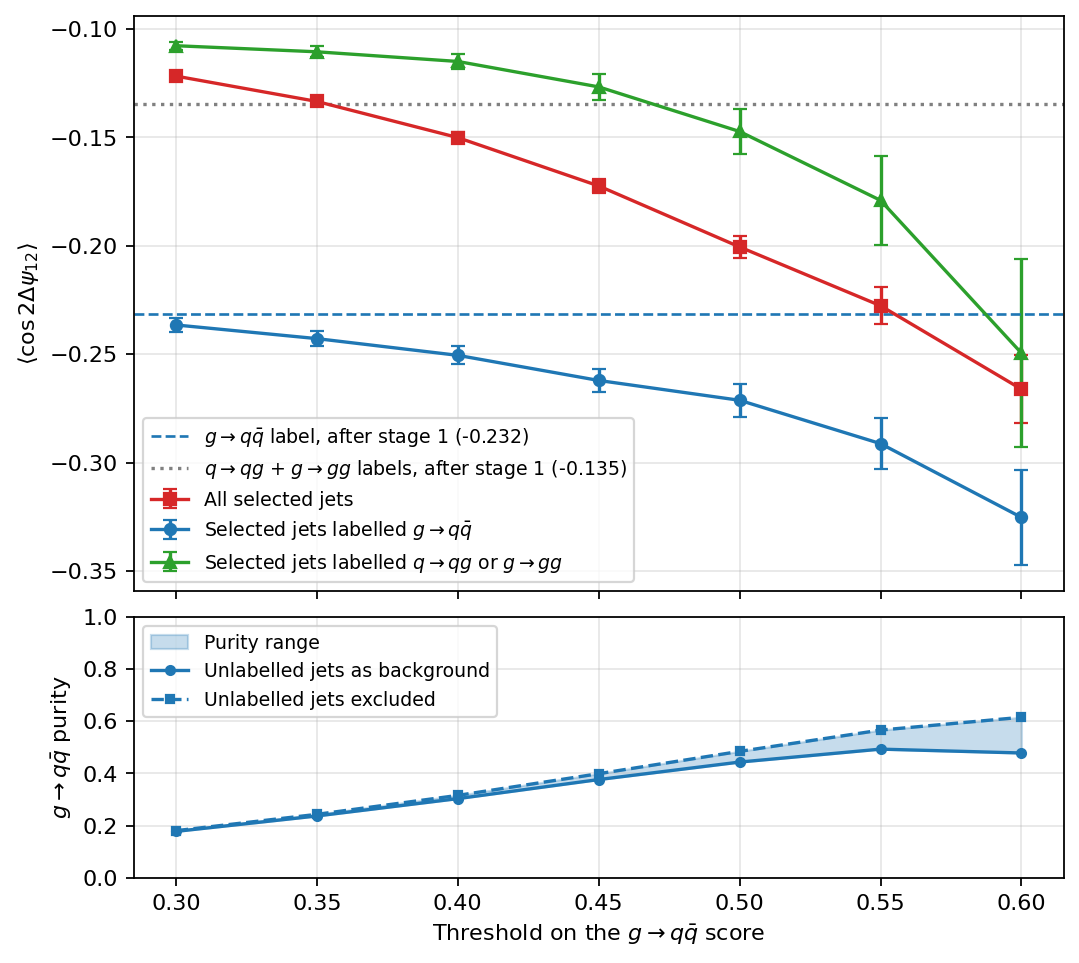
\includegraphics[width=0.7\textwidth]{figuras/modulation_components.png}
  \caption{Top: mean value $\langle \cos 2\dpsi \rangle$ of all jets selected by
  the two-stage selection in the simulated calibration sample, and of the selected
  jets labelled $g \to q\bar{q}$ and labelled $q \to qg$ or $g \to gg$, as a
  function of the threshold on the $g \to q\bar{q}$ score. All jets have a matched
  score above $0.8$. The horizontal lines show the mean values of the two classes
  with this requirement alone, without any threshold on the second score. Bottom:
  purity of the selected samples, with the jets without channel label counted as
  background and excluded, respectively.}
  \label{fig:modulation-components}
\end{figure}

The two purities coincide up to a threshold of about $0.45$, which shows that the
selected samples contain almost no jets without channel label at low thresholds.
The selection as a whole therefore strongly disfavours these jets, which make up
$31\%$ of the inclusive sample. At higher thresholds, however, the purities become
notably separated, and at a threshold of $0.60$ a fifth of the selected jets carry
no label. The tightest requirements thus retain proportionally more jets without a
generator-level counterpart, which causes the purity counting them as background
to saturate at about $0.5$.

The behaviour of the selection is further clarified by following the jets of the signal
and background classes separately. Among the jets passing the requirement on the
matched score, those labelled $g \to q\bar{q}$ have a mean value of
$-0.232 \pm 0.003$, and those labelled $q \to qg$ or $g \to gg$ a mean value of
$-0.135 \pm 0.001$. Within the selection, the jets labelled $g \to q\bar{q}$ become
steadily more negative as the threshold increases, from $-0.237 \pm 0.003$ at
$0.30$ to $-0.325 \pm 0.022$ at $0.60$. However, the background classes also become 
more negative as the threshold increases, from $-0.108 \pm 0.002$ at $0.30$ to $-0.249 \pm 0.043$
at $0.60$, and the decrease accelerates at the highest thresholds. At the lowest
thresholds their mean value lies above the reference of $-0.135$, which shows that
the first requirement on the second score removes background configurations with
a stronger than average modulation. The curve crosses the reference at a threshold
of about $0.47$, and at $0.60$ the background approaches the signal, although these
channels carry no or a slightly positive spin correlation. Therefore, 
the selection enriches the sample in the $g \to q\bar{q}$ channel and also
favours, at its tightest requirements, configurations in which the modulation 
is stronger whatever their channel.

Nevertheless, the difference between the two classes is still notable. Between
thresholds of $0.30$ and $0.50$, the jets labelled $g \to q\bar{q}$ lie between
$0.12$ and $0.14$ below the background selected at the same threshold. The
difference decreases only at the highest thresholds, to $0.11$ at $0.55$ and
$0.08 \pm 0.05$ at $0.60$, where both classes are dominated by the effect of the
selection. If the selection shifted the modulation of all channels by the same amount, this
shift would cancel in the difference between them, which would then remain
constant even as both classes become more negative. This is what is observed up to
a threshold of $0.50$. The stability of the difference therefore indicates that,
beyond the common effect of the selection, the $g \to q\bar{q}$ channel carries a
modulation of its own, about $0.13$ stronger than that of the background. At the
highest thresholds the difference decreases, which suggests that the effect of
the selection is no longer the same for all channels.

\subsection{Kinematics of the selected splittings}
\label{sec:res-mod-z}

The selection acts on the kinematics of each splittings as well as on their
flavour. The splitting function of equation~\eqref{eq:Pgq} favours symmetric
$g \to q\bar{q}$ splittings, in contrast with those of $g \to gg$ and $q \to qg$,
which are enhanced when one of the two products is soft. The distribution of the
momentum fraction $z_2$ of the second splitting is shown in the left panel of
Figure~\ref{fig:z-kinematics}. As one can notice, both classes rise towards $z_2 = 1/2$, since the
splitting of largest $\kt$ is selected in each sequence and $\kt$ grows with $z$.
However, their shapes are different. With jets below $z_2 \approx 0.3$ the channels
$q \to qg$ and $g \to gg$ are relatively more frequent, while above that those labelled
$g \to q\bar{q}$ are more frequent. The selection amplifies this effect, and with it,
at a threshold of $0.60$, almost no selected jet has $z_2 < 0.25$, and the distribution rises much
more steeply up to $z_2 = 1/2$. 

\begin{figure}[htbp]
  \centering
  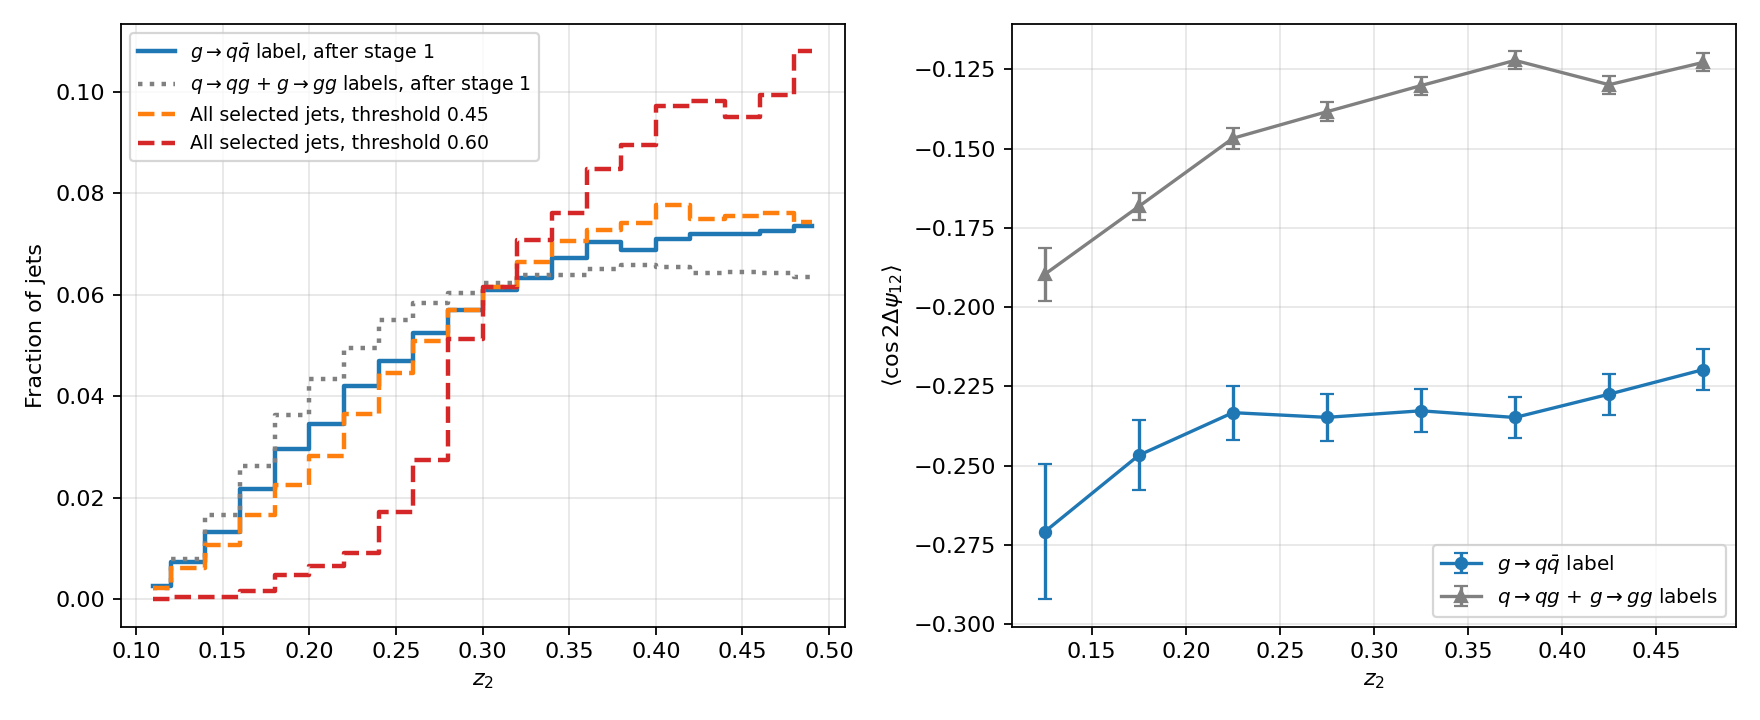
\includegraphics[width=\textwidth]{figuras/z_kinematics.png}
  \caption{Left: distribution of the momentum fraction $z_2$ of the second
  splitting for the jets labelled $g \to q\bar{q}$ and for those labelled
  $q \to qg$ or $g \to gg$ after the first stage, and for all jets selected at
  thresholds of $0.45$ and $0.60$, normalised to unit area. Right: mean value
  $\langle \cos 2\dpsi \rangle$ as a function of $z_2$ for the jets labelled
  $g \to q\bar{q}$ and for those labelled $q \to qg$ or $g \to gg$ after the first
  stage. All results are obtained on the simulated calibration sample.}
  \label{fig:z-kinematics}
\end{figure}

The dependence of the modulation on $z_2$ is shown in the right plot. For the background,
the modulation is most negative for asymmetric
splittings, $-0.19$ at $z_2 \approx 0.12$, and weakens to about $-0.12$ for
symmetric ones. These channels should carry no or a positive spin correlation, 
thus these reveals a component of the modulation that is not of spin
origin and is strongest for asymmetric splittings. For the jets labelled
$g \to q\bar{q}$ the modulation is instead nearly independent of $z_2$, at about
$-0.23$ over most of the range, whereas at leading order in the collinear limit
the spin correlation of this channel grows strongly towards symmetric
splittings~\cite{Karlberg_2021}. The difference between the two classes, which
removes the component common to both, grows from about $0.08$ for asymmetric
splittings to about $0.11$ for symmetric ones. It thus follows the expected
direction, but varies much less than predicted. This discrepancy is discussed in
Section~\ref{sec:res-discussion}.

These results explain part of the behaviour of Section~\ref{sec:res-mod-sim}. The
first requirements on the second score remove mainly background splittings with
low $z_2$, which carry the strongest modulation, so that the selected background
initially lies above its reference. The shift towards symmetric splittings cannot,
however, explain the strengthening of the modulation at the highest thresholds,
since symmetric splittings show a weaker modulation in the background and an
essentially unchanged one in the $g \to q\bar{q}$ class. Weighting the modulation
of each class by the distribution of $z_2$ of the jets selected at $0.60$ would
give about $-0.23$ for the $g \to q\bar{q}$ class and $-0.13$ for the background,
far from the observed values of $-0.325 \pm 0.022$ and $-0.249 \pm 0.043$. This
strengthening must therefore arise from other properties of the splittings to
which the classifier is sensitive, such as the momentum fraction of the first
splitting, the opening angles or the shapes of the branches, whose identification
is left for future work.

\subsection{Comparison with collision data}
\label{sec:res-mod-data}

The same selection procedure is applied to the collision data with the same networks
trained on simulation and the same requirements on both scores. The mean value
$\langle \cos 2\dpsi \rangle$ of the selected jets is compared with that of the
simulated calibration sample in Figure~\ref{fig:modulation-data}, however, 
the collision data is much smaller. At a threshold of $0.30$ it contains $2\,607$ jets, about $110$
times fewer than the $286\,380$ simulated ones, and only $162$, $50$ and $16$ jets
remain at $0.50$, $0.55$ and $0.60$. Therefore, the statistical uncertainty
of the data dominates the comparison at every threshold. Nevertheless,
the fraction of jets at low threshold are very similar between the two samples, by at most about $15\%$, 
which shows that the score distributions of data and simulation are close.

\begin{figure}[htbp]
  \centering
  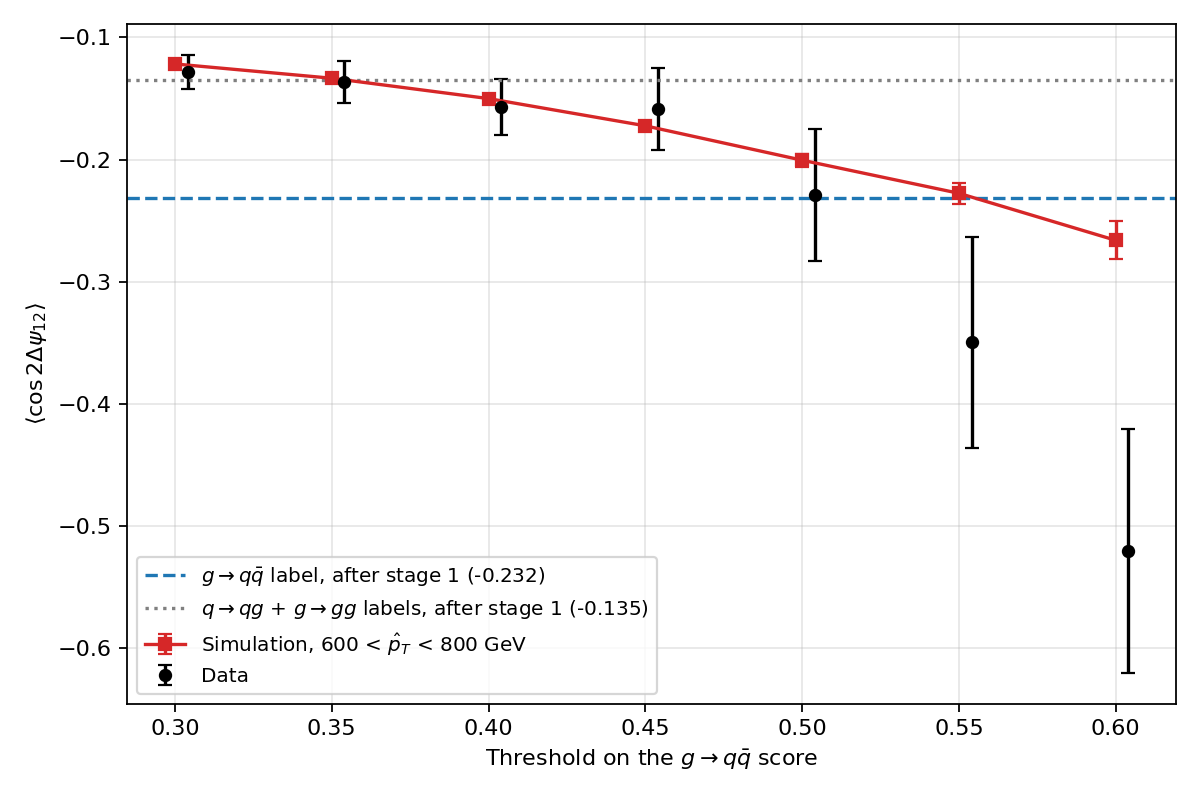
\includegraphics[width=0.7\textwidth]{figuras/modulation_threshold.png}
  \caption{Mean value $\langle \cos 2\dpsi \rangle$ of the jets selected by the
  two-stage selection as a function of the threshold on the $g \to q\bar{q}$
  score, in the collision data and in the simulated calibration sample. All jets
  have a matched score above $0.8$. The horizontal lines show the mean values in
  simulation of the jets labelled $g \to q\bar{q}$ and of those labelled
  $q \to qg$ or $g \to gg$ after this requirement alone. The data points are
  shifted slightly to the right for readability, and the error bars show the
  statistical uncertainties.}
  \label{fig:modulation-data}
\end{figure}

The quantitive comparison is restricted to thresholds up to $0.50$ since, in this range,
the data sample contains more than $150$ jets, and its statistical
uncertainty is at most about half of the difference of $0.097$ between the two
reference values. With thresholds above this value the uncertainty becomes comparable to this difference,
and the data can no longer distinguish a sample dominated by $g \to q\bar{q}$
splittings from one dominated by background.

Then, at thresholds below $0.5$, the mean values agree within less than one standard deviation, from
$-0.128 \pm 0.014$ in data and $-0.122 \pm 0.001$ in simulation at $0.30$ to
$-0.229 \pm 0.054$ and $-0.201 \pm 0.005$ at $0.50$. Thus, the modulation in data strenghtens
with the threshold, just like in simulation. Since the selected samples are
grouped together, the jets selected at $0.50$ are also part of the sample at $0.30$, and the
uncertainty of the change between the two thresholds is approximately
$\sqrt{\sigma_{0.50}^2 - \sigma_{0.30}^2}$, smaller than the combination of the two
uncertainties. Between $0.30$ and $0.50$ the mean value in data decreases by
$0.101 \pm 0.052$, compared with $0.079$ in simulation. Therefore, the strengthening is
seen in data with a significance of about two standard deviations.

However, above the threshold of $0.50$, the data lies below the simulation, by $1.4$ standard deviations at
$0.55$ and by $2.5$ at $0.60$, where the mean value reaches $-0.52 \pm 0.10$. These
two points rest on very few jets and are strongly correlated. The $16$ jets
selected at $0.60$ are also part of the $50$ selected at $0.55$, and the remaining
$34$ jets, with scores between $0.55$ and $0.60$, have a mean value of about
$-0.27$, in agreement with the simulation. The deviation at both thresholds
therefore comes mostly from the $16$ jets of highest score. With so few jets the
Gaussian approximation of the uncertainty is itself unreliable, and the central
value at $0.60$ even lies beyond $-1/2$, the most negative value allowed by a
modulation of the form of equation~\eqref{eq:dpsi-modulation}. This illustrates the
size of the statistical fluctuations at these thresholds, and a deviation of this
kind in the last of several correlated points is not evidence of a disagreement
with simulation.

Within the precision of the data, it is possible to say that it describes both
the response of the selection and the modulation of the selected jets. However this
agreement does not establish the presence of spin correlation in data, since 
part of the strengthening of the modulation in simulation is common to all
channels and is induced by the selection itself, as shown in
Section~\ref{sec:res-mod-sim}, and no simulated sample without spin correlations is
available to isolate the contribution of spin origin. These points are discussed
in Section~\ref{sec:res-discussion}.

\section{Three-point energy correlator}
\label{sec:res-eeec}

The three-point energy correlator of Section \ref{sec:eeec-impl} gives a second probe of
the spin correlations, built directly from jet constituents and independent of the declustering.
Its distribution in the azimuthal angle $\psi$ is computed over
all triplets of constituents inside the window of equation \eqref{eq:eeec-window}, each
with the weight of equation \eqref{eq:eeec-weight}, and normalised to unit area over
$(-\pi,\pi]$. Its modulation is summarised by the weighted mean

\begin{equation}
  \langle \cos 2\psi \rangle =
  \frac{\sum_{\text{jets}} \sum_{abc} w_{abc} \cos 2\psi_{abc}}
       {\sum_{\text{jets}} \sum_{abc} w_{abc}} ,
  \label{eq:eeec-mean}
\end{equation}

which is related to the coefficients of a modulation of the form of
equation \eqref{eq:dpsi-modulation} by $a_2/a_0 = 2\langle \cos 2\psi \rangle$, as for
$\dpsi$. The constituents of a jet share elements with one another and are therefore 
not independent, thus, statistical uncertainties are calculated by treating the jets 
as the independent units. Since the simulated calibration dataset is much larger than 
the collision dataset, the distributions of all jets
are obtained from the first $5 \times 10^{5}$ events which makes 
the statistical uncertainty much smaller than that of the data while the latter uses 
all selected events. For the labelled classes in the simulated calibration dataset,
all events were used.

The distribution of all jets is shown in the left panel of Figure \ref{fig:eeec-distributions}.
This distribution reveals a clear modulation, symmetric under $\psi \to -\psi$ as 
expected from parity invariance, with maxima at $\psi = 0$ and $\pm\pi$ and minima at $\pm\pi/2$.
The mean values obtained are $+0.020 \pm 0.001$ in data and
$+0.019 \pm 0.001$ in simulation, which is equivalent to $a_2/a_0 \approx +0.04$,
and the ratio of data to simulation is compatible with unity within about $2\%$ in
every bin. The shape is closer to a single $\cos 2\psi$ harmonic, with, however,
a minima somewhat deeper than this harmonic would produce, as it is possible to
see when comparing to the red dashed line. With this, the obtained distribution 
has positive sign and thus it is opposite to that of the inclusive $\dpsi$
distribution of Section~\ref{sec:res-inclusive}, and about four times smaller in
magnitude.

\begin{figure}[htbp]
  \centering
  \begin{minipage}{0.49\textwidth}
    \centering
    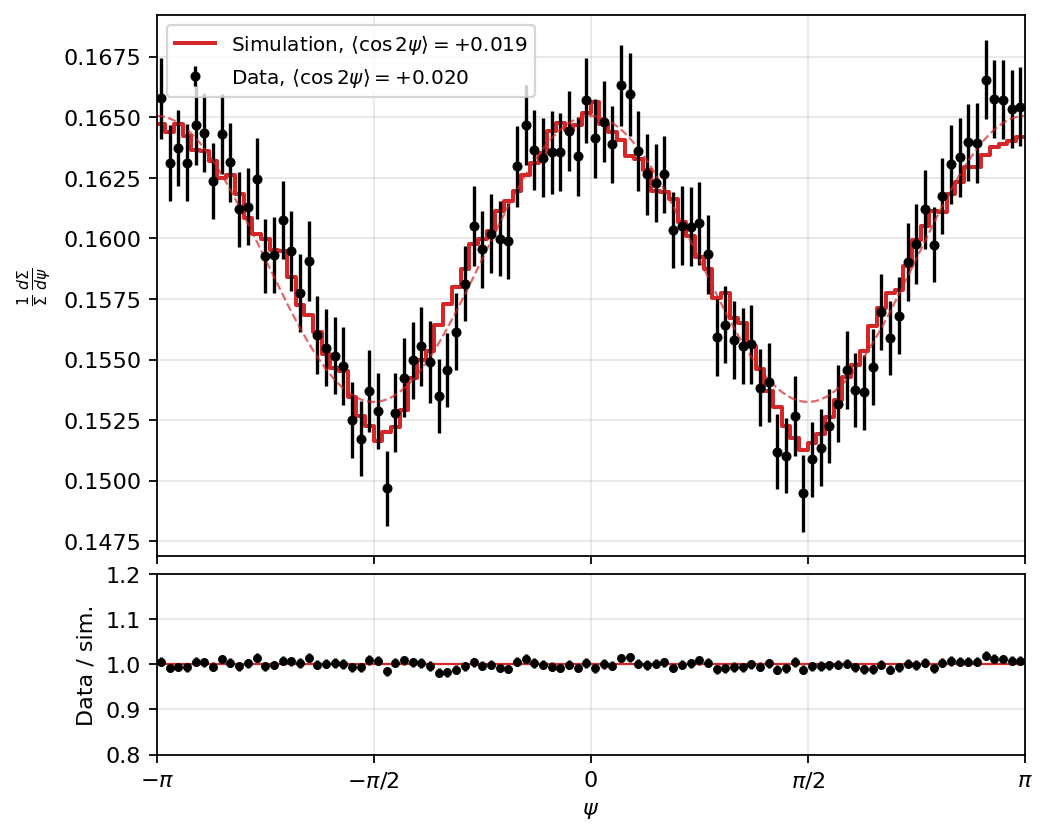
\includegraphics[width=\textwidth]{figuras/eeec_inclusive.png}
  \end{minipage}\hfill
  \begin{minipage}{0.49\textwidth}
    \centering
    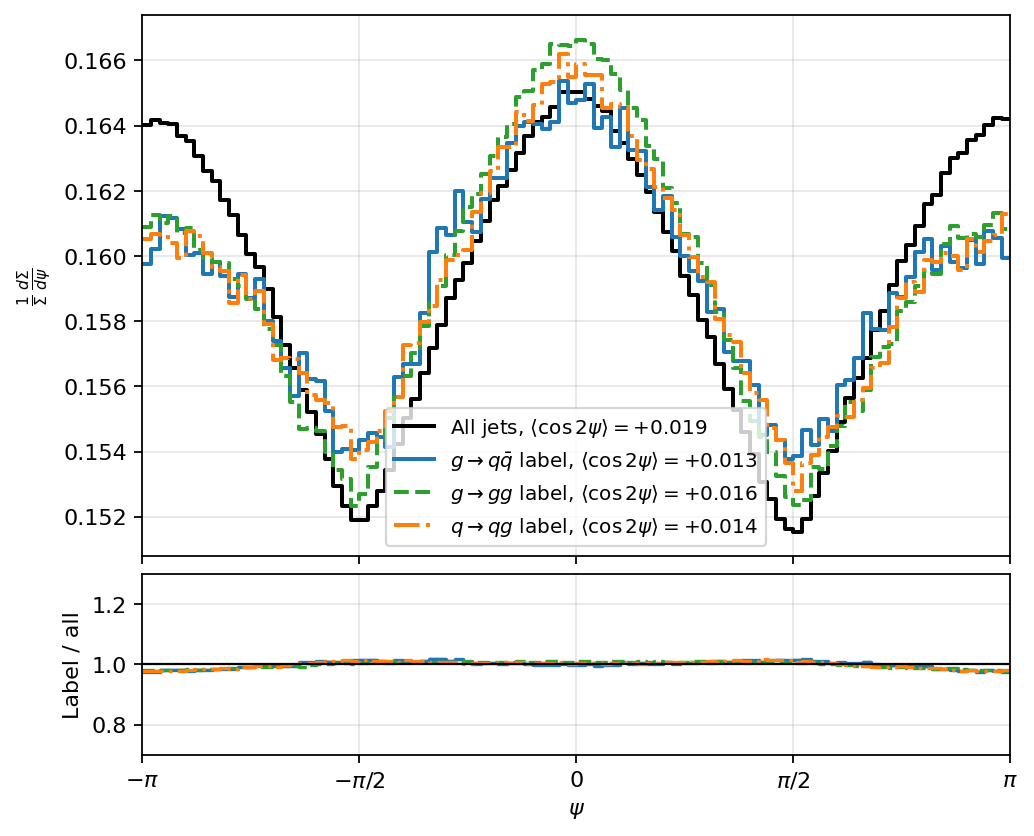
\includegraphics[width=\textwidth]{figuras/eeec_labels.png}
  \end{minipage}
  \caption{Distribution of the azimuthal angle $\psi$ of the three-point energy
  correlator, normalised to unit area. The left panel compares all jets in the
  collision data and in the simulated calibration sample, with the ratio of data
  to simulation in the lower panel. The right panel shows the simulated jets
  labelled $g \to q\bar{q}$, $g \to gg$ and $q \to qg$ together with all simulated
  jets, with the ratio of each class to all jets in the lower panel. The dashed
  line in the left panel is the pure $\cos 2\psi$ modulation with the mean value
  of the simulation.}
  \label{fig:eeec-distributions}
\end{figure}

The right panel of Figure \ref{fig:eeec-distributions} shows the seperation by channel label,
and demonstrates almost no dependence on the channel. All channels demonstrate a positive 
modulation of close size. The mean value is $+0.0125 \pm 0.0006$ for the
jets labelled $g \to q\bar{q}$, $+0.0136 \pm 0.0004$ for $q \to qg$ and
$+0.0161 \pm 0.0002$ for $g \to gg$, and the distributions of the three classes
differ from that of all jets by at most about $3\%$ in every bin. The jets of
the $g \to q\bar{q}$ channel have the weakest positive modulation and 
they differ from the other classes by less than $0.004$. In comparison with the
$\dpsi$ modulation, the same label has a much negative modulation, as shown in Section~\ref{sec:res-labelling}.
This main difference between the observables happens because of how they are built. The channel
label corresponds to the second splitting of the Lund declustering, while the three-point energy
correlator sums over every triplet inside a fixed angular window, most of which do not
resolve that splitting. Therefore, a jet with a labelled channel of $g \to q\bar{q}$
mainly contributes to the correlator through triplets unrelated to its $g \to q\bar{q}$ splitting.
The mean value of all jets, $+0.019 \pm 0.001$, is larger than that of
every labelled class because it is dominated by the unmatched jets and by those
without a label. These make up almost $90\%$ of the jets and have mean values of
$+0.0200$ and $+0.0196$.

The labelled channels also show a feature that is much weaker in the sample with all jets. 
Their maximum at $\psi = \pm\pi$ is about $3\%$ lower than that at
$\psi = 0$, which corresponds to a term in $\cos\psi$. Exchanging the two closest
constituents $a$ and $b$ reverses the normal $\hat{n}_1$ of
equation \eqref{eq:eeec-normals} and shifts $\psi$ by $\pi$. Therefore, the distinction between
$\psi = 0$ and $\psi = \pm\pi$ depends on which of the two is taken as
$a$, here the one stored first. A term of this kind does not have the period $\pi$
of the spin correlation and does not contribute to $\langle \cos 2\psi \rangle$.

The three-point energy correlator of the jets selected by the flavour selection procedure are shown
in Figure \ref{fig:eeec-threshold} as a function of the threshold. After passing the first 
selection stage and the requirement of having a matched score above $0.8$, 
the jets labelled $g \to q\bar{q}$ and the
background have mean values of $+0.010$ and $+0.012$, which differ by only $0.002$,
compared with about $0.10$ for $\dpsi$. Therefore, using the networks to enrich the samples
with the $g \to q\bar{q}$ label can barely change the correlator. Nevertheless, in simulation
the mean value decreases steadily with the threshold, from about
$+0.014$ at $0.30$ to about $+0.001$ at $0.60$, and it lies outside the range
spanned by the two references at both ends. Its size, about $0.013$, is however an order of
magnitude smaller than the corresponding change of $\dpsi$ seen in Section~\ref{sec:res-mod-sim}.
The data follow the
simulation. Up to a threshold of $0.50$, the range retained in
Section~\ref{sec:res-mod-data}, they differ from it by at most about $1.3$ standard
deviations, from $+0.017 \pm 0.004$ against $+0.014$ at $0.30$ to
$-0.007 \pm 0.021$ against $+0.010$ at $0.50$. Above this threshold the
uncertainty of the data exceeds the whole variation of the simulation.

\begin{figure}[htbp]
  \centering
  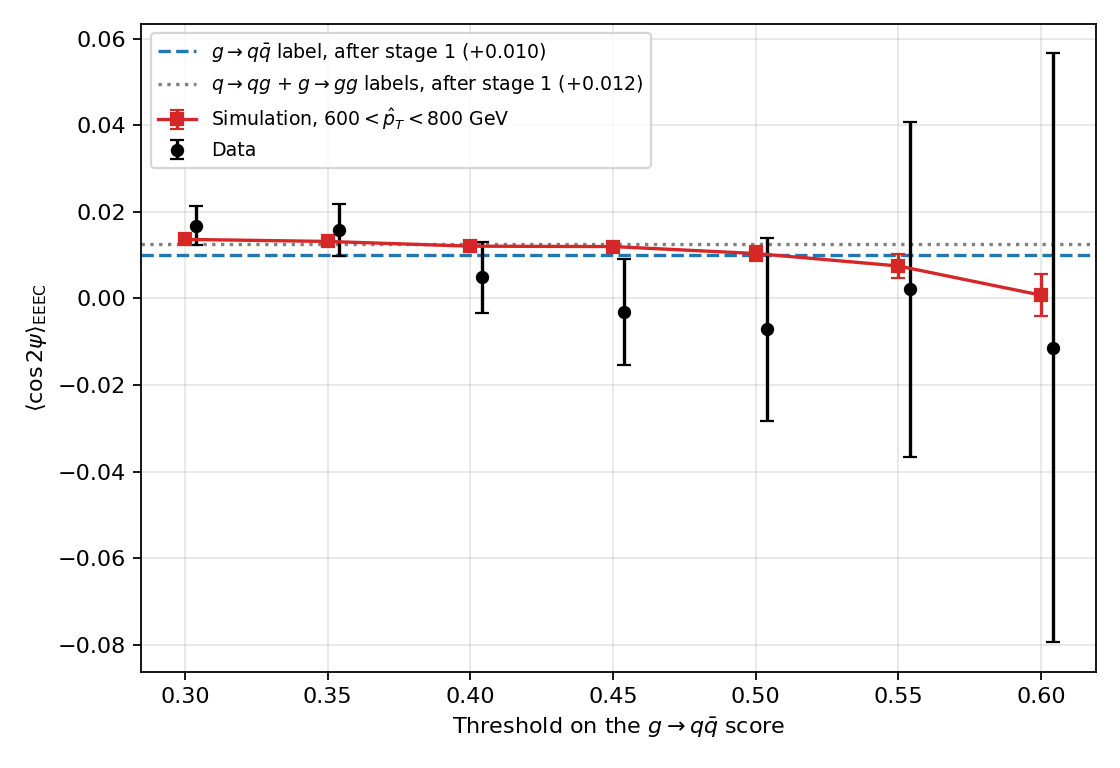
\includegraphics[width=0.6\textwidth]{figuras/eeec_threshold.png}
  \caption{Mean value $\langle \cos 2\psi \rangle$ of the three-point energy
  correlator of the jets selected by the two-stage selection as a function of the
  threshold on the $g \to q\bar{q}$ score, in the collision data and in the
  simulated calibration sample. All jets have a matched score above $0.8$. The
  horizontal lines show the mean values in simulation of the jets labelled
  $g \to q\bar{q}$ and of those labelled $q \to qg$ or $g \to gg$ after this
  requirement alone. The data points are shifted slightly to the right for
  readability, and the error bars show the statistical uncertainties.}
  \label{fig:eeec-threshold}
\end{figure}

Thus, the three-point energy correlator shows a modulation that the simulation follows the
collision data, although with a positive sign, nearly insensitive to the channel
labelling of the Lund declustering, and only weakly affected by a flavour selection
built on the declustering. It does not reproduce the strong negative modulation
associated with $g \to q\bar{q}$ splittings in the $\dpsi$ observable. These
results are compared with the theoretical expectations of
\cite{Karlberg_2021} in Section~\ref{sec:res-discussion}.

\section{Discussion}
\label{sec:res-discussion}

The previous sections presented the computation of the two spin-sensitive
observables in collision data and simulation, before and after flavour selection.
This section interprets these results, compares them with the theoretical
expectations of \cite{Karlberg_2021}, obtained at second order in the
collinear limit for electron-positron collisions, and with the CMS
measurement~\cite{CMS:2026jnt}, which observed the spin correlations in
$g \to q\bar{q}$ splittings with an analysis similar to the present one. 

The discussion is organised in four parts. Section~\ref{sec:disc-theory} examines
whether the observed modulations have the properties expected from spin
correlations. Section~\ref{sec:disc-selection} discusses the effect of the flavour
selection on the modulation, and Section~\ref{sec:disc-cms} the comparison with
the CMS measurement. Section~\ref{sec:disc-limits} summarises the limitations of
the analysis that follow from these comparisons.

\subsection{Comparison with theoretical expectations}
\label{sec:disc-theory}

In simulation, the jets labelled as $g \to q\bar{q}$ revealed the most negative modulation,
$\langle \cos 2\dpsi \rangle = -0.167 \pm 0.002$, but with half the magnitude of the collinear prediction of, $-0.31$. 
A weaker modulation is, although, expected 
for several reasons. The IFN label is a flavour proxy and does not
coincide splitting by splitting with the vertex of the parton shower.
The observable was built from reconstructed, after hadronisation and detector effects.
The prediction also refers to quark-initiated jets in electron-positron collisions. This
work is done in proton-proton collisions and a large fraction of the jets are initiated by gluons,
which the intermediate gluon is produced in a
$g \to gg$ splitting with a different degree of polarisation, so no prediction
specific to proton--proton collisions is available for $\dpsi$.

A larger deviation appears on the classes which little or no spin correlation is expected.
The jets, with labels $g \to gg$ and $q \to qg$, have mean values of
$-0.077$ and $-0.091$, where the predictions are $+0.025$ and zero, and the
unmatched jets have $-0.059$. For all jets together, the inclusive value of
$-0.083$ in simulation and $-0.078$ in data compares with a prediction of about
$-0.013$. Thus, a negative component of the modulation is present on each channel.
Two of its properties are visible in the results.
It depends strongly on the kinematics of the second splitting and is largest for
asymmetric splittings, as shown in Section~\ref{sec:res-mod-z}. It is also
accompanied by higher harmonics in the inclusive distribution of
Section~\ref{sec:res-inclusive}, whereas a collinear spin correlation at this
order contributes only a $\cos 2\dpsi$ term. Both properties suggest an origin in
the kinematics of the declustering rather than in the spin of the intermediate
gluon. The simulation reproduces this component in data, so it is described by the
generator and the detector simulation, but its origin is not identified in this
work. Its dominance is consistent with the CMS measurement, in which switching off the
spin correlations in \textsc{Pythia}~8 changes the inclusive distribution of
$\dpsi$ by only about $0.5\%$~\cite{CMS:2026jnt}.

Since this component is common to all classes, the difference between the
$g \to q\bar{q}$ class and the background is the quantity closest to the spin
correlation of the $g \to q\bar{q}$ channel. Before any selection it amounts to
$0.086$, from $-0.167$ and $-0.081$, and after the first stage of the selection to
$0.097$, from $-0.232$ and $-0.135$. Both values are less than a third of the
difference of about $0.33$ between the predictions for the $g \to q\bar{q}$ and
$g \to gg$ channels. Also, the dependence of this difference on $z_2$ is much weaker
than expected. At leading order, the azimuthal dependence of the
$g \to q\bar{q}$ splitting of a linearly polarised gluon is proportional to
$1 - 2z(1-z) - 2z(1-z)\cos 2\phi$, so that its analysing power,
$2z(1-z)/[1 - 2z(1-z)]$, grows from $0.22$ at $z_2 = 0.1$ to $1$ at $z_2 = 1/2$.
The difference computed instead grows from about $0.08$ below $z_2 = 0.2$ to about
$0.10$ above $z_2 = 0.3$. This may be either the non-spin
component does not cancel completely in the difference, or the spin correlation
is strongly diluted at reconstruction level because of the smearing of $z_2$,
the cases where the reconstructed splitting does not correspond to the
generator-level one, and by those in which
the label does not correspond to the channel of the shower. 
The two effects cannot be separated without a reference in
which the spin correlations are absent, as discussed in
Section~\ref{sec:disc-cms}.

The three-point energy correlator departs further from the expectations. 
For quark-initiated jets in electron-positron collisions, In \cite{Karlberg_2021} predicts mean
values $\langle \cos 2\psi \rangle$ of about $-0.18$ for the $g \to q\bar{q}$
channel, $+0.013$ for $g \to gg$ and $-0.004$ for all jets together. The result 
obtained here in this work is positive, $+0.0186 \pm 0.0001$ in simulation and
$+0.0200 \pm 0.0012$ in data, and it depends little on the channel label. The jets
labelled $g \to q\bar{q}$, with $+0.0125 \pm 0.0006$, differ from those labelled
$g \to gg$ by only $0.004$. The weak dependence on the label follows may come from 
the construction of the correlator, which sums over all triplets inside a fixed window
and thus not tied to the second splitting of the declustering, as
discussed in Section~\ref{sec:res-eeec}. The positive sign is not explained here, but
it may reflect the larger fraction of gluon-initiated jets at a hadron collider,
whose $g \to gg$ splittings contribute positively, the transposition of the
angular window from electron-positron collisions to the $(\eta,\phi)$ plane, or a
non-spin component of the same kind as the one found for $\dpsi$. However,
the present work does not discriminate between these possibilities.

\subsection{Effect of the flavour selection}
\label{sec:disc-selection}

The flavour selection developed in this work strengthens the modulation of the selected jets from
$-0.122$ at a threshold of $0.30$ to $-0.266$ at $0.60$, while the purity rises
from about $0.18$ to between $0.48$ and $0.62$. If the selection only changed the proportions
of the channels, the jets of each class would keep the modulation they have after
the first stage, $-0.232$ for the $g \to q\bar{q}$ class and $-0.135$ for the
background, and the mean value of the labelled jets would lie between these two
values. So, at a threshold of $0.60$, where the observed purity was at most $0.62$, 
such a mixture would give a modulation of $-0.19$. However, at this threshold,
the labelled jets selected have instead a mean value of about $-0.30$, more negative than the reference of
the $g \to q\bar{q}$ class itself.

Thus, the modulation of each class changes with the threshold. The jets labelled
$g \to q\bar{q}$ become more negative, from $-0.237$ to $-0.325$, and the jets
labelled $q \to qg$ or $g \to gg$ even more so, from $-0.108$ to $-0.249$,
even though their label does not change. There are two possible explanations, and
they are not exclusive. The first one is that the classifier, which does not use $\dpsi$ as an
input, selects configurations in which the non-spin component of the modulation 
identified in Section~\ref{sec:disc-theory} is stronger, through features
correlated with it. Part of this effect is explained by the momentum fraction of
the second splitting, as shown in Section~\ref{sec:res-mod-z}. The second one 
is that the shift reflects the limitations of the IFN label. The label does not
coincide splitting by splitting with the vertex of the parton shower, and the classifier,
trained on the substructure of the branches, may recognise real
$g \to q\bar{q}$ splittings better than the label does. At high thresholds, the jets 
with the label of $g \to q\bar{q}$ would then mostly be those in which the label is
correct, and the jets labelled as background would increasingly be
$g \to q\bar{q}$ splittings that the label assigns to another channel. Thus,
both would carry a stronger spin correlation, and the true purity would be
higher than the purity defined by the IFN label. The mean value of the
jets labelled $g \to q\bar{q}$ at the highest threshold, $-0.325 \pm 0.022$, close
to the prediction of $-0.31$, is consistent with this interpretation. As argued in
Section~\ref{sec:disc-theory}, however, the negative modulation of the background
before any selection cannot be attributed to such splittings.

The difference between the two classes stays close to $0.13$ from a threshold of
$0.30$ up to $0.50$, and decreases to $0.076 \pm 0.049$ at $0.60$. According to the
first explanation, the common shift cancels in this difference, and, according to the second one,
decrease at the highest thresholds would reflect the growing fraction of genuine
$g \to q\bar{q}$ splittings among the jets labelled as background, although it is
not significant within the statistical uncertainties. Unfortunately, the two explanations
cannot be separated with the samples available in this work. They would differ only on
a sample where no spin correlations are present, in which the first would still produce 
a shift and the second would not, and in the dependence of the additional modulation on
$z_2$, which should grow towards symmetric splittings if it is of spin origin. In
either case, the mean value of the selected sample combines the enrichment in
$g \to q\bar{q}$ splittings with effects that cannot be separated from it in data.
For this reason, the result is presented as a function of the threshold, and not instead 
as a function of the purity. A linear extrapolation of the modulation
to a purity of one would assume that the modulations of the signal and of the
background do not depend on the threshold, and the simulation shows that this
assumption does not hold.

The comparison with the collision data is subject to the same limitation. Between thresholds of
$0.30$ and $0.50$ the modulation in data strengthens by $0.101 \pm 0.052$,
compared with $0.079$ in simulation. Therefore, the collision data follows the simulation,
but this agreement holds whichever of the two
explanations applies, and it does not distinguish between them.

The energy correlator also behaves in a similar way. Its mean value decreases with the
threshold by about $0.013$ for all selected jets and by a similar amount for those
labelled $g \to q\bar{q}$, from $+0.0093$ to $-0.0017$, although the two labelled
references after the first stage differ by only $0.0025$. Therefore,
the selection changes the correlator
mainly through properties of the selected jets other than their label.

\subsection{Comparison with the CMS measurement}
\label{sec:disc-cms}

The CMS measurement used $34.7$~fb$^{-1}$ of proton-proton collisions recorded in
2022 at $\sqrt{s} = 13.6$~TeV~\cite{CMS:2026jnt}. The distribution of $\dpsi$ in
the selected jets was compared with the predictions of \textsc{Pythia}~8 and
\textsc{Herwig}~7, each with and without the angular correlations induced by the
gluon spin. The hypothesis without correlations is disfavoured with an observed
significance of $6.8$ standard deviations, for an expected $8.1$, while the data
differ from the hypothesis with correlations by $1.9$ standard deviations and
favour a slightly weaker modulation than predicted. Its strategy is very close to the
one followed here.
The composition of the simulated samples is very similar, as shown in
Section~\ref{sec:res-labelling}. The purity reached by CMS, $38\%$ for a score
above $0.6$ in its four-class network, is also of the same order as the purities
obtained here, from $0.38$-$0.40$ at a threshold of $0.45$ to $0.44$-$0.49$ at
$0.50$, although the two analyses define the purity with different matching
criteria.

Nevertheless the two analysis differ in several aspects. CMS reconstructs jets
using the PUPPI algorithm for pileup mitigation, while the jets in this work 
are corrected with charged-hadron subtraction, and it applies the requirements on
the constituents and on the second subjet discussed in
Section~\ref{sec:sys-choices}. CMS' classifier has four classes and is trained on
the \textsc{Herwig}~7 sample without spin correlations, so that it cannot exploit
the modulation itself. Here the selection is performed in two stages and trained
on a \textsc{Pythia}~8 sample. However, the four-class network studied as an
alternative in Section~\ref{sec:res-performance} performs comparably to the
two-stage selection, so that the choice of architecture is not expected to be the
main difference between the two results.

The decisive difference lies in the predictions against which the data are
compared. In CMS, the predictions with and without spin correlations are processed
through the same selection, so that every effect of the selection that does not
originate from the spin is present in both and cancels in their comparison. These
predictions also show how small the spin-induced part of the modulation is. In
\textsc{Pythia}~8, switching off the correlations changes the inclusive
distribution by only about $0.5\%$, and the distribution of the selected
$g \to q\bar{q}$ category by at most $12\%$~\cite{CMS:2026jnt}. This is consistent
with the large non-spin component found in Section~\ref{sec:disc-theory}, which
the selection does not remove. The same comparison would also separate the two
explanations of Section~\ref{sec:disc-selection}, since a shift caused by the
selection of the non-spin component would persist without spin correlations,
whereas a shift caused by genuine $g \to q\bar{q}$ splittings assigned to other
channels would disappear.

In \textsc{Pythia}~8 the correlations are included as an average modulation of the
angle between the production and splitting planes of the
gluon~\cite{CMS:2026jnt}, and the nominal sample used here therefore corresponds
to a prediction with correlations. The agreement between data and simulation found
in Section~\ref{sec:res-mod-data} is thus consistent with the CMS observation that
the data agree with \textsc{Pythia}~8 with correlations. No sample without spin
correlations is available among the CMS Open Data simulations of the period
studied here, however, so this agreement cannot be turned into a statement on the
presence of spin correlations in the data. A numerical comparison of the
modulation itself is not possible either, since CMS presents the distribution of
$\dpsi$, at detector and at particle level, but not its mean value
$\langle \cos 2\dpsi \rangle$. The present analysis thus reproduces the strategy of
the CMS measurement with public data from an earlier period, but cannot by itself
reach its conclusion. What it adds is a decomposition of the modulation by channel
class in simulation, which shows how the flavour selection acts on each class and
why the modulation of the selected samples cannot be interpreted as that of the
$g \to q\bar{q}$ channel alone.

\subsection{Limitations}
\label{sec:disc-limits}

The main limitations of this analysis come from the preceding subsections. The 
most important is the absence of a simulation without spin correlations. The simulation
used here includes the approximate treatment of the correlations of
\textsc{Pythia}~8, and the CMS measurement shows that the spin-induced part of the
modulation is small compared with the non-spin component. Without a reference using 
the same selection, but with
the correlations are turned off, the two components cannot be separated, and neither can the two
explanations of the effect of the selection discussed in
Section \ref{sec:disc-selection}.

This analysis also relies on a single generator. \textsc{Pythia}~8 with the CP5
tune is used for the training of the classifier, for the calibration of the
selection, for the determination of the purity and for the comparison with data.
The dependence of the composition and of the purity on the description of the
parton shower and of the hadronisation is therefore not tested, as discussed in
Section~\ref{sec:sys-purity}. This dependence is likely to be relevant, since
\textsc{Pythia}~8 and \textsc{Herwig}~7 treat the spin correlations differently
and predict different strengths of the modulation \cite{CMS:2026jnt}.

The computed purity is defined through the IFN label, which is a flavour proxy
assigned through an angular matching. About $31\%$ of the simulated jets carry no label,
which is why the purity is quoted in an interval, and the true fractions
of $g \to q\bar{q}$ splittings in the selected samples may differ from the labelled
one, as discussed in Section~\ref{sec:disc-selection}.

The collision data correspond to a single period of data taking, with about
$4.6 \times 10^{4}$ jets with a valid $\dpsi$. Their statistical precision limits
the comparison with simulation to thresholds up to $0.50$, and it is insufficient
to resolve differences of the size expected between predictions with and without
spin correlations. All results are also obtained at detector level, without
correction for the resolution and acceptance of the detector, so their comparison
with theoretical predictions is only qualitative. Finally, only statistical
uncertainties are given. The systematic sources of Section~\ref{sec:systematic}
are not propagated, and the analysis choices that differ from the CMS
measurement, discussed in Section~\ref{sec:sys-choices}, are not varied.

Within these limitations, the analysis shows that the full chain, from the
released data to a flavour-enriched measurement of the modulation, can be carried
out with public data and tools. It also shows that the simulation describes the
data well in the observables central to this work, namely the plane
$(z_1, z_2)$, the modulation as a function of the threshold and the energy
correlator. The extensions needed to turn this agreement into a statement on the
presence of spin correlations are discussed in Chapter~\ref{cap:conclusoes}.
\chapter{Conclusions}
\label{cap:conclusoes}

\section{Summary of the results}
\label{sec:conc-summary}

This work studied the collinear spin correlations in QCD jets with CMS Open Data datasets, using 
two observables sensitive to the polarisation of an intermediate gluon. The first 
computed observable is the azimuthal angle $\dpsi$ between the planes of two
successive splittings of the Lund declustering. The second is the azimuthal
modulation of the three-point energy correlator. Both of them were measured 
in jets with $\pt > 700$~GeV in the 2016 collision data and compared with the corresponding
\textsc{Pythia}~8 simulation, before and after a flavour selection designed to
enrich the samples in $g \to q\bar{q}$ splittings. The results are summarised below 
in relation to the objectives of Section~\ref{sec:objetivos}.

A fully complete and reproducible analysis was developed over the released data. It
extracts the jets and their constituents information inside the CMS software environment, and
performs the declustering, the generator-level labelling of the splittings, the
computation of the energy correlator and the flavour selection outside it, with
public tools. The simulation describes the collision data kinematics, and the primary and secondary Lund jet planes
show the structure expected from the emission pattern of QCD and from the
boundaries set by the grooming condition and by the jet radius. The momentum fractions 
distributions of the two selected splittings agree between data and simulation as well, 
with mean values of $0.270$ and $0.283$ in data
against $0.268$ and $0.283$ in simulation.

The observed $\dpsi$ shows a clear $\cos(2\dpsi)$ modulation even before any flavour selection,
with $\langle \cos 2\dpsi \rangle = -0.078 \pm 0.003$ in data and
$-0.083$ in simulation. In simulation, the jets labelled as $g \to q\bar{q}$ have a
modulation about twice as strong as the background, $-0.167$ against $-0.081$,
with a negative sign as predicted for this channel. However, every channel carries a negative
modulation, including those in which little or no spin correlation is
expected. This non-spin component is largest for asymmetric splittings and
dominates the inclusive modulation, in line with the small difference between
the \textsc{Pythia}~8 predictions with and without spin correlations reported by
CMS. The three-point energy correlator also shows a modulation that the simulation describes
well in data, $+0.0200 \pm 0.0012$ against $+0.0186 \pm 0.0001$, but it has a positive sign 
and is almost independent of the channel, in contradiction with the theory prediction.
In the configuration used here,
it is therefore not a channel-selective probe of the spin correlations.

A two-stage flavour selection was developed, in which a first network separates
matched from unmatched splittings and a second network identifies the
$g \to q\bar{q}$ channel among the matched ones. This selection raises the purity 
of the selected samples from $0.03$ before any selection to between $0.48$ and $0.62$ at
the highest threshold. It performs best among the methods studied at low
efficiency, while a four-class network developed as an alternative test, similar to the one used by CMS, is better
at high efficiency. The purity counted against all jets saturates at about $0.5$,
because the tightest requirements retain proportionally more jets without a
generator-level counterpart. This sets the practical limit of the selection with
the features used.

Using this selection, the modulation of the selected jets strengthens steadily with
the threshold, from $-0.122$ at $0.30$ to $-0.266$ at $0.60$ in simulation. The data 
follows the simulation within one standard deviation up to a threshold of
$0.50$, beyond which their statistical precision is insufficient. However,
a modulation of a pure $g \to q\bar{q}$ sample could not be established. The modulation of each
labelled class changes with the threshold, so the selected samples do not behave
as mixtures of classes with fixed modulations,
and a linear extrapolation to a purity of one is not justified. The most reasonable
quantity is the difference between the $g \to q\bar{q}$ class and the background,
which stays close to $0.13$ up to a threshold of $0.50$, and which is less than 
half of the difference expected at leading order. The shift present in both classes can be explained
by a selection of configurations with a stronger non-spin
component, or by genuine $g \to q\bar{q}$ splittings that the label assigns to
other channels. Despite of these hypothesis, the samples available do not allow 
them to be studied or tested.

The sources of systematic uncertainties were identified, with those related to the purity 
limiting the interpretation most. These are the dependence of
the purity on the generator and on the definition of the channel label.
However, the most important limitation of this work is the absence of a simulated dataset 
without spin correlations processed using the selection adopted here. A dataset of that 
kind allowed CMS to establish the presence of the correlations, and it is not
available among the released simulations of the period studied. Nevertheless, the present
analysis reproduces the strategy of the CMS measurement with public data,
and its results are consistent with the CMS observation that the data agree with
\textsc{Pythia}~8 with spin correlations, although, it cannot establish by itself 
their presence. Its main contribution is the decomposition of the modulation by channel
class, which shows that the modulation of a flavour-selected sample cannot be
interpreted as that of the $g \to q\bar{q}$ channel alone. This applies to any
measurement of this kind, and it supports comparing the data with predictions
without spin correlations rather than interpreting the selected modulation
directly.

\section{Future work}
\label{sec:conc-future}

The most important extension would be a prediction without spin correlations, 
processed with the same selection as in data. In \textsc{Pythia}~8 the correlations can
be switched off in the parton shower, and \textsc{Herwig}~7 treats them explicitly
through the spin-density matrix, so that samples with and without correlations can
be generated with both. A full simulation of the CMS detector is computationally
demanding, but a first study can be carried out at particle level, where the
flavour selection, the labelling and the observables can be applied without
change. Such samples would separate the spin and non-spin components of the
modulation, and would distinguish between the two explanations of the effect of
the selection discussed in Section~\ref{sec:disc-selection}.

The flavour selection procedure could also be improved in two directions.
Although $\dpsi$ is not an input of the classifier, the shift that the selection induces in every
class shows that its score is correlated with $\dpsi$ through other features. Training another
classifier explicitly decorrelated from $\dpsi$, using, for instance, a penalty
on the distance correlation between its score and
$\dpsi$~\cite{Kasieczka:2020disco} or with an adversarial network~\cite{Louppe:2017pivot}, 
would limit this shift, possibly at the cost of
some discriminating power. Another and a simpler solution would be training the network
on a sample without spin correlations, as done by CMS. This would also ensure that any
residual correlation would not originate from spin. The dependence of the purity on the definition of the channel label
should also be studied, by comparing the matching of the two branches of the
second splitting used here with alternatives such as the matching of subjets 2 and
3 used by CMS. A second generator would finally test how much the composition and
the purity depend on the description of the parton shower and of the
hadronisation.

On the collision data side, the statistical precision could be increased by using 
other datasets of other periods of the 2016 data taking available in CMS Open Data.
This would permit a comparison with simulation at the highest thresholds. The
systematic uncertainties identified in Section~\ref{sec:systematic} should be
propagated to the results, and the analysis choices that differ from the CMS
measurement, in particular the thresholds on the transverse momentum of the
constituents and of the second subjet, should be varied. An unfolding of the
measured distributions to particle level would finally allow a direct comparison
with theoretical predictions and with the CMS result.

The three-point energy correlator requires a different treatment in order to become 
sensitive to the $g \to q\bar{q}$ channel. Its angular window was transposed from
electron-positron collisions, and its optimisation for jets at a hadron collider,
together with predictions for proton-proton collisions, would clarify the origin
of the positive modulation observed here. Restricting the triplets to the
constituents of the branches selected by the Lund declustering would also tie the
correlator to the labelled splitting, and allow the flavour selection to act on
it in the same way as on $\dpsi$.

Concluding, this analysis chain is not restricted to proton-proton collisions.
CMS also released heavy-ion data, in which the same observables 
could be used to study whether the spin correlations of the parton shower are
modified by the quark-gluon plasma. However the simulated heavy-ion datasets, that 
are suitable for this analysis, do not include jet quenching and their maximum
jet radius is at maximum of $R=0.5$. Nevertheless,
they can provide a reference without medium effects, but not a prediction of how
the medium modifies the correlations, which would require dedicated samples
generated with a model of jet quenching. The reference provided by the
proton-proton measurement, together with the understanding of the selection
obtained in this work, is a necessary starting point for such a study.

\cleardoublepage
\printbibliography[heading=bibintoc,title={REFERENCES}]

\appendix
%\include{capitulos/anexo-a}
\chapter{Supplementary Numerical Results}
\label{anexo:b}

This appendix collects the numerical values behind the figures of
Chapter~\ref{cap:resultados} that are not tabulated in the main text. The tables
follow the order in which the results are presented there, and all uncertainties
are statistical.

\begin{table}[htbp]
  \centering
  \caption{Number of jets with a valid $\dpsi$, mean values of the momentum
  fractions $z_1$ and $z_2$ of the two selected splittings, and correlation
  coefficient between them, for all jets in the collision data and in the
  simulated calibration sample, and for the simulated jets in each class of the
  channel label of the second splitting. The fraction is given relative to all
  simulated jets. The statistical uncertainties are below $0.001$ for the mean
  values and below $0.005$ for the correlation coefficients.}
  \label{tab:zplane}
  \begin{tabular}{lrrccc}
    \toprule
    Sample & Jets & Fraction & $\langle z_1 \rangle$ & $\langle z_2 \rangle$ & $\rho(z_1, z_2)$ \\
    \midrule
    Data, all jets & $45\,755$ & & $0.270$ & $0.283$ & $-0.032$ \\
    \midrule
    Simulation, all jets & $8\,495\,207$ & $100.0\%$ & $0.268$ & $0.283$ & $-0.031$ \\
    \quad no label & $2\,647\,865$ & $31.2\%$ & $0.267$ & $0.285$ & $-0.026$ \\
    \quad unmatched & $4\,397\,983$ & $51.8\%$ & $0.264$ & $0.275$ & $-0.028$ \\
    \quad $g \to q\bar{q}$ & $179\,810$ & $2.1\%$ & $0.275$ & $0.315$ & $-0.064$ \\
    \quad $q \to qg$ & $358\,498$ & $4.2\%$ & $0.294$ & $0.294$ & $-0.066$ \\
    \quad $g \to gg$ & $857\,140$ & $10.1\%$ & $0.273$ & $0.301$ & $-0.086$ \\
    \quad rest & $53\,911$ & $0.6\%$ & $0.299$ & $0.305$ & $-0.048$ \\
    \bottomrule
  \end{tabular}
\end{table}

\begin{table}[htbp]
  \centering
  \caption{Performance of the first stage of the flavour selection as a function of
  the threshold on the matched score, evaluated on the test set of the training
  sample. Among the labelled splittings of this set, a fraction $0.234$ is matched.
  The purity is the fraction of matched splittings among those selected, the
  efficiency is the fraction of matched splittings that are selected, and the last
  column gives the fraction of unmatched splittings that are selected. The
  threshold of $0.8$ is the one adopted in this work.}
  \label{tab:stage1-scan}
  \begin{tabular}{ccccc}
    \toprule
    Threshold & Selected fraction & Purity & Efficiency & Unmatched selected \\
    \midrule
    $0.30$ & $0.449$ & $0.427$ & $0.820$ & $0.336$ \\
    $0.40$ & $0.323$ & $0.516$ & $0.714$ & $0.204$ \\
    $0.50$ & $0.241$ & $0.599$ & $0.618$ & $0.126$ \\
    $0.60$ & $0.184$ & $0.672$ & $0.530$ & $0.079$ \\
    $0.70$ & $0.143$ & $0.733$ & $0.449$ & $0.050$ \\
    $0.75$ & $0.123$ & $0.764$ & $0.403$ & $0.038$ \\
    $\mathbf{0.80}$ & $\mathbf{0.102}$ & $\mathbf{0.797}$ & $\mathbf{0.349}$ & $\mathbf{0.027}$ \\
    $0.85$ & $0.080$ & $0.830$ & $0.284$ & $0.018$ \\
    $0.90$ & $0.054$ & $0.865$ & $0.198$ & $0.009$ \\
    $0.95$ & $0.012$ & $0.917$ & $0.046$ & $0.001$ \\
    \bottomrule
  \end{tabular}
\end{table}

\begin{table}[htbp]
  \centering
  \caption{Mean value $\langle \cos 2\dpsi \rangle$ of the jets selected by the
  two-stage selection as a function of the threshold on the $g \to q\bar{q}$
  score, in the simulated calibration sample and in the collision data. All jets
  have a matched score above $0.8$. The purity is given as the interval between
  the values obtained by counting the jets without a channel label as background and
  excluding them. In simulation, the mean value is given for all selected jets,
  for those labelled $g \to q\bar{q}$, and for those labelled $q \to qg$ or
  $g \to gg$. After the requirement on the matched score alone, these two labelled
  classes have mean values of $-0.2315 \pm 0.0027$ and $-0.1346 \pm 0.0011$. The
  uncertainties are statistical.}
  \label{tab:modulation-scan}
  \footnotesize
  \setlength{\tabcolsep}{4pt}
  \begin{tabular}{crccccrc}
    \toprule
    & \multicolumn{5}{c}{Simulation} & \multicolumn{2}{c}{Data} \\
    \cmidrule(lr){2-6} \cmidrule(l){7-8}
    & & & \multicolumn{3}{c}{$\langle \cos 2\dpsi \rangle$} & & \\
    \cmidrule(lr){4-6}
    Threshold & Jets & Purity & All selected & $g \to q\bar{q}$ & $q \to qg$, $g \to gg$
              & Jets & $\langle \cos 2\dpsi \rangle$ \\
    \midrule
    $0.30$ & $286\,380$ & $0.179$--$0.181$ & $-0.1218 \pm 0.0013$ & $-0.2365 \pm 0.0030$ & $-0.1078 \pm 0.0018$ & $2\,607$ & $-0.1281 \pm 0.0138$ \\
    $0.35$ & $165\,321$ & $0.238$--$0.244$ & $-0.1335 \pm 0.0017$ & $-0.2428 \pm 0.0034$ & $-0.1106 \pm 0.0025$ & $1\,613$ & $-0.1366 \pm 0.0174$ \\
    $0.40$ & $90\,503$  & $0.304$--$0.316$ & $-0.1501 \pm 0.0023$ & $-0.2505 \pm 0.0041$ & $-0.1150 \pm 0.0036$ & $924$    & $-0.1568 \pm 0.0231$ \\
    $0.45$ & $42\,982$  & $0.377$--$0.399$ & $-0.1724 \pm 0.0034$ & $-0.2621 \pm 0.0053$ & $-0.1268 \pm 0.0059$ & $423$    & $-0.1585 \pm 0.0336$ \\
    $0.50$ & $18\,220$  & $0.444$--$0.485$ & $-0.2006 \pm 0.0052$ & $-0.2712 \pm 0.0075$ & $-0.1473 \pm 0.0105$ & $162$    & $-0.2289 \pm 0.0539$ \\
    $0.55$ & $6\,548$   & $0.493$--$0.566$ & $-0.2276 \pm 0.0085$ & $-0.2912 \pm 0.0118$ & $-0.1791 \pm 0.0204$ & $50$     & $-0.3495 \pm 0.0864$ \\
    $0.60$ & $1\,852$   & $0.478$--$0.615$ & $-0.2661 \pm 0.0156$ & $-0.3252 \pm 0.0221$ & $-0.2495 \pm 0.0433$ & $16$     & $-0.5202 \pm 0.0997$ \\
    \bottomrule
  \end{tabular}
\end{table}

\begin{table}[htbp]
  \centering
  \caption{Mean value $\langle \cos 2\dpsi \rangle$ as a function of the momentum
  fraction $z_2$ of the second splitting, for the simulated jets labelled
  $g \to q\bar{q}$ and for those labelled $q \to qg$ or $g \to gg$, after the
  requirement of a matched score above $0.8$. The last column gives the
  difference between the two classes. The values correspond to the right panel
  of Figure~\ref{fig:z-kinematics}, and the uncertainties are statistical.}
  \label{tab:z-profile}
  \begin{tabular}{cccc}
    \toprule
    $z_2$ & $g \to q\bar{q}$ & $q \to qg$ or $g \to gg$ & Difference \\
    \midrule
    $0.10$--$0.15$ & $-0.2709 \pm 0.0213$ & $-0.1896 \pm 0.0084$ & $-0.0813 \pm 0.0229$ \\
    $0.15$--$0.20$ & $-0.2467 \pm 0.0110$ & $-0.1682 \pm 0.0042$ & $-0.0785 \pm 0.0118$ \\
    $0.20$--$0.25$ & $-0.2333 \pm 0.0085$ & $-0.1467 \pm 0.0033$ & $-0.0866 \pm 0.0091$ \\
    $0.25$--$0.30$ & $-0.2348 \pm 0.0074$ & $-0.1383 \pm 0.0030$ & $-0.0965 \pm 0.0080$ \\
    $0.30$--$0.35$ & $-0.2327 \pm 0.0068$ & $-0.1301 \pm 0.0029$ & $-0.1026 \pm 0.0074$ \\
    $0.35$--$0.40$ & $-0.2348 \pm 0.0065$ & $-0.1222 \pm 0.0028$ & $-0.1126 \pm 0.0071$ \\
    $0.40$--$0.45$ & $-0.2275 \pm 0.0064$ & $-0.1298 \pm 0.0028$ & $-0.0977 \pm 0.0070$ \\
    $0.45$--$0.50$ & $-0.2197 \pm 0.0064$ & $-0.1228 \pm 0.0029$ & $-0.0969 \pm 0.0070$ \\
    \bottomrule
  \end{tabular}
\end{table}

\begin{table}[htbp]
    \centering
    \caption{Mean value $\langle \cos 2\psi \rangle$ of the three-point energy
    correlator for all jets in the collision data and in the simulated calibration
    sample, and for the simulated jets in each class of the channel label of the
    second splitting. All jets of the ntuples are included, also those without a
    valid $\dpsi$. The last two rows give the labelled classes used as references in
    Figure~\ref{fig:eeec-threshold}, after the requirement of a matched score above
    $0.8$ alone. The coefficient of the modulation is
    $a_2/a_0 = 2\langle \cos 2\psi \rangle$. The uncertainties are statistical and
    treat the jets as independent.}
    \label{tab:eeec-classes}
    \begin{tabular}{lrrc}
      \toprule
      Sample & Jets & Triplets & $\langle \cos 2\psi \rangle$ \\
      \midrule
      Data, all jets & $60\,566$ & $1.54 \times 10^{8}$ & $+0.0200 \pm 0.0012$ \\
      \midrule
      Simulation, all jets & $11\,476\,817$ & $2.58 \times 10^{10}$ & $+0.0186 \pm 0.0001$ \\
      \quad no label & $5\,629\,475$ & $5.21 \times 10^{9}$ & $+0.0196 \pm 0.0002$ \\
      \quad unmatched & $4\,397\,983$ & $1.35 \times 10^{10}$ & $+0.0200 \pm 0.0001$ \\
      \quad $g \to q\bar{q}$ & $179\,810$ & $7.18 \times 10^{8}$ & $+0.0125 \pm 0.0006$ \\
      \quad $q \to qg$ & $358\,498$ & $1.73 \times 10^{9}$ & $+0.0136 \pm 0.0004$ \\
      \quad $g \to gg$ & $857\,140$ & $4.36 \times 10^{9}$ & $+0.0161 \pm 0.0002$ \\
      \quad rest & $53\,911$ & $2.79 \times 10^{8}$ & $+0.0130 \pm 0.0010$ \\
      \midrule
      Matched score $> 0.8$, $g \to q\bar{q}$ & $64\,104$ & $3.24 \times 10^{8}$ & $+0.0100 \pm 0.0009$ \\
      Matched score $> 0.8$, $q \to qg$ or $g \to gg$ & $388\,308$ & $2.70 \times 10^{9}$ & $+0.0125 \pm 0.0003$ \\
      \bottomrule
    \end{tabular}
  \end{table}
  
  \begin{table}[htbp]
    \centering
    \caption{Mean value $\langle \cos 2\psi \rangle$ of the three-point energy
    correlator of the jets selected by the two-stage selection, as a function of
    the threshold on the $g \to q\bar{q}$ score, in the collision data and in the
    simulated calibration sample. All jets have a matched score above $0.8$. The
    last two columns refer to the selected simulated jets labelled
    $g \to q\bar{q}$. The uncertainties are statistical and treat the jets as
    independent.}
    \label{tab:eeec-threshold}
    \small
    \begin{tabular}{crcrcrc}
      \toprule
      & \multicolumn{2}{c}{Data}
      & \multicolumn{2}{c}{Simulation, all selected}
      & \multicolumn{2}{c}{Simulation, $g \to q\bar{q}$ label} \\
      \cmidrule(lr){2-3} \cmidrule(lr){4-5} \cmidrule(l){6-7}
      Threshold & Jets & $\langle \cos 2\psi \rangle$
                & Jets & $\langle \cos 2\psi \rangle$
                & Jets & $\langle \cos 2\psi \rangle$ \\
      \midrule
      $0.30$ & $2\,607$ & $+0.0168 \pm 0.0046$ & $286\,380$ & $+0.0136 \pm 0.0004$ & $51\,186$ & $+0.0093 \pm 0.0010$ \\
      $0.35$ & $1\,613$ & $+0.0158 \pm 0.0061$ & $165\,321$ & $+0.0132 \pm 0.0006$ & $39\,305$ & $+0.0093 \pm 0.0011$ \\
      $0.40$ & $924$    & $+0.0049 \pm 0.0082$ & $90\,503$  & $+0.0121 \pm 0.0008$ & $27\,512$ & $+0.0095 \pm 0.0014$ \\
      $0.45$ & $423$    & $-0.0032 \pm 0.0122$ & $42\,982$  & $+0.0120 \pm 0.0011$ & $16\,197$ & $+0.0082 \pm 0.0018$ \\
      $0.50$ & $162$    & $-0.0071 \pm 0.0211$ & $18\,220$  & $+0.0104 \pm 0.0017$ & $8\,084$  & $+0.0044 \pm 0.0026$ \\
      $0.55$ & $50$     & $+0.0021 \pm 0.0387$ & $6\,548$   & $+0.0075 \pm 0.0027$ & $3\,229$  & $+0.0035 \pm 0.0040$ \\
      $0.60$ & $16$     & $-0.0114 \pm 0.0679$ & $1\,852$   & $+0.0008 \pm 0.0048$ & $886$     & $-0.0017 \pm 0.0073$ \\
      \bottomrule
    \end{tabular}
  \end{table}

\end{document}
